\section{Tutorial: Hola Gatito}
\label{sec:tutor-hola-gatito}

Típicamente el primer programa que se realiza para probar un nuevo
computador o lenguaje de programación muestra el mensaje ``Hola
Mundo'' para mostrar que todo está conectado y funcionando
correctamente. En \AppInventor incluso las aplicaciones más simples
pueden hacer mucho más que sólo mostrar mensajes: ellas pueden
reproducir sonidos y reaccionar cuando el usuario toca el
dispositivo. Así que vamos a comenzar con algo mucho más emocionante:
tu primera aplicación se llamará \appName{Hola Gatito}. En general
todas las aplicaciones se definen por sus pantallas visibles---lo que
se conoce como la \textit{interfaz de usuario}---y su
comportamiento. La pantalla de la aplicación se muestra en
la~\Cref{fig:holaGatito}, y su comportamiento será como sigue:

\begin{itemize}
\item \whenDo{la imagen es presionada}{se emite el sonido de un
    maullido y el dispositivo vibra.}
\item \whenDo{el dispositivo es agitado}{se emite el sonido de un maullido.}
\end{itemize}

\begin{figure}[H]
\centering
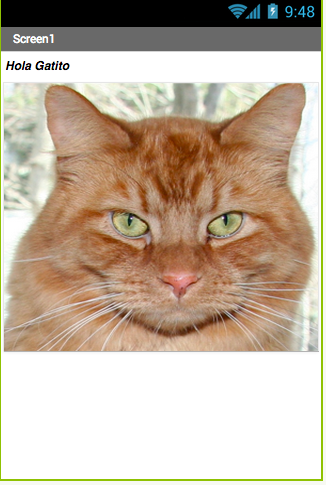
\includegraphics[scale=0.3]{HolaGatito}
\caption{Pantalla de aplicación \appName{Hola Gatito}}
\label{fig:holaGatito}
\end{figure}

\subsection*{Qué Aprenderás}

Siguiendo este tutorial aprenderás a:

\begin{itemize}

\item Construir aplicaciones en \AppInventor seleccionando componentes
  y diciéndoles qué hacer y cuándo hacerlo.

\item Usar el \componentDesigner para seleccionar componentes. Algunos
  componentes son visibles en la pantalla del dispositivo mientras que
  otros no lo son.

\item Agregar archivos multimedia (sonidos e imágenes) a las
  aplicaciones, subiéndoles a \AppInventor desde tu computador.

\item A usar el \blockEditor para ensamblar bloques de código que
  definen el comportamiento de los componentes, y que por lo tanto en
  conjunto definen el comportamiento de la aplicación.

\item Probar las aplicaciones directamente en los dispositivos, lo que
  te ayudará a ver cómo las aplicaciones se comportan, paso a paso, a
  medida que las construyes.

\item Empaquetar las aplicaciones que construyes para instalarlas en
  un dispositivo.

\end{itemize}

\subsection*{El Ambiente de Desarrollo \AppInventor}

Para comenzar a programar con App Inventor debes acceder al sitio
\aiurl.\footnote{Necesitas una cuenta de Google para utilizar
  \AppInventor} Esto abrirá la última versión de App Inventor,
publicada en Diciembre de 2013. Algunas personas llaman a esta
aplicación App Inventor 2, pero su nombre formal sigue siendo App
Inventor, y la versión anterior se conoce como App Inventor
Classic. Nosotros usaremos siempre la nueva versión.  El entorno de
programación App Inventor tiene 3 partes esenciales:

\begin{itemize}

\item El \componentDesigner, que se muestra en la~\Cref{fig:componentDesigner}. Se usa para seleccionar los componentes de la
  aplicación y especificar sus propiedades.

\item El \blockEditor, que se muestra en la~\Cref{fig:blockEditor}. Se
  usa para especificar cómo se comportan los componentes (por ejemplo,
  qué pasa cuando se presiona un botón).

\item Un dispositivo Android que te permite ejecutar y probar las
  aplicaciones a medida que las vas desarrollando. Si no tienes un
  dispositivo Android disponible, puedes probar las aplicaciones
  usando el Emulador Android. Como en el taller utilizaremos teléfonos
  móviles no nos preocuparemos de cómo instalar y usar el emulador
  (igual puedes consultar a tu tutor cómo hacerlo, si quieres
  programar en tu casa).

\end{itemize}

\begin{figure}[H]
\centering
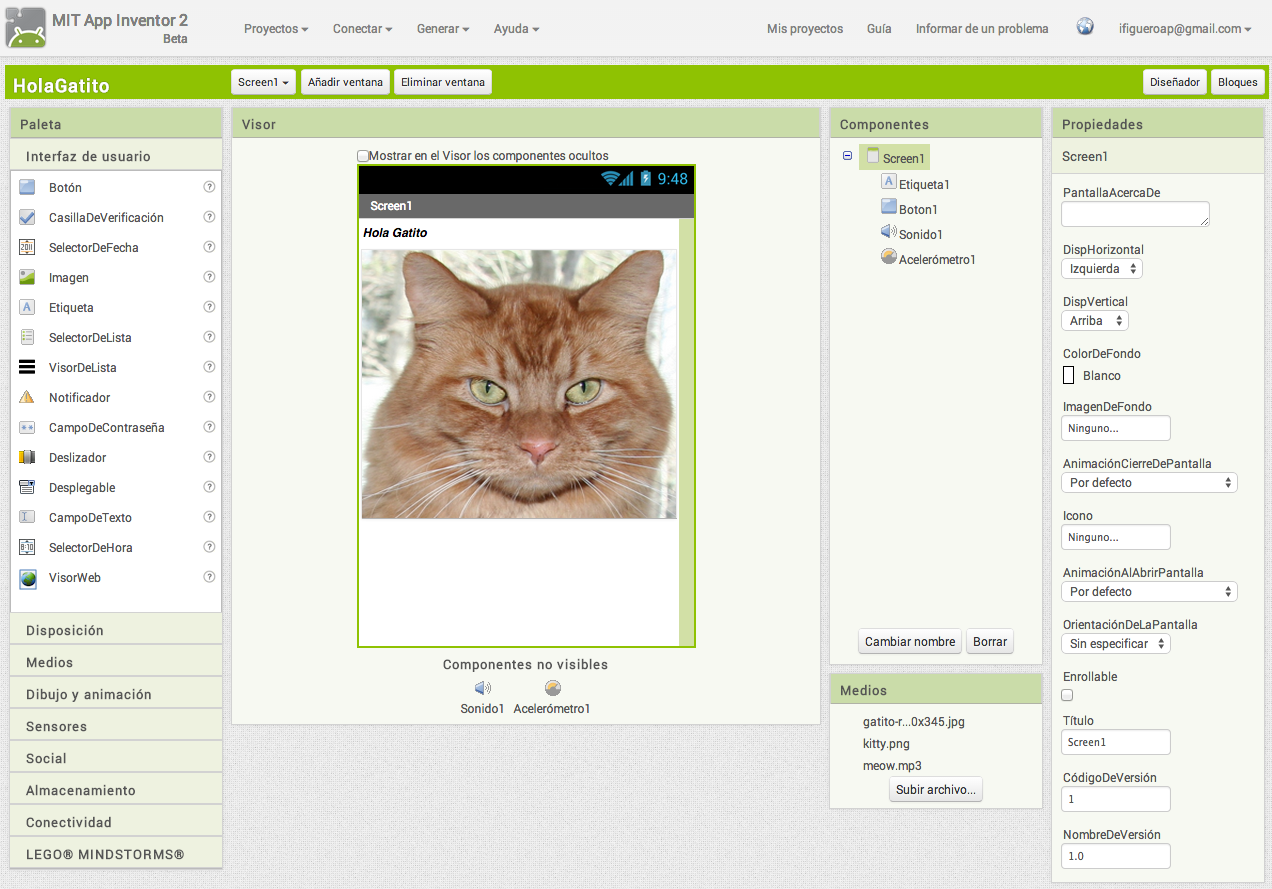
\includegraphics[scale=0.25]{componentDesigner}
\caption{\componentDesigner}
\label{fig:componentDesigner}
\end{figure}

\begin{figure}[H]
\centering
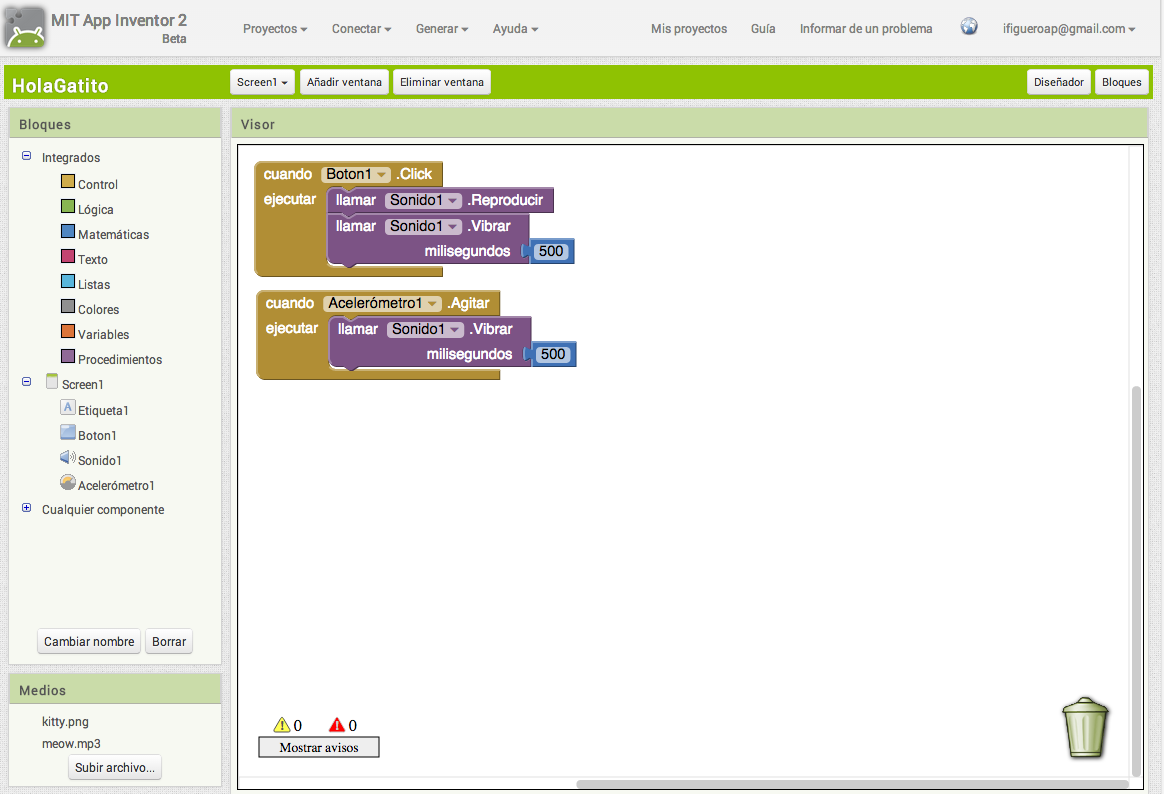
\includegraphics[scale=0.25]{blockEditor}
\caption{\blockEditor}
\label{fig:blockEditor}
\end{figure}

La primera vez que ingreses a \aiurl, verás la página de Proyectos, la
que seguramente estará en blanco porque aún no has creado ningún
proyecto. Para crear un proyecto, presiona el botón ``Comenzar un
proyecto nuevo'' en la esquina superior izquierda de la página,
ingresa el nombre ``HolaGatito'' (los nombres de proyecto son sin
espacios), y luego presiona ``Aceptar''. La~\Cref{fig:crearProyecto}
muestra la creación del proyecto \appName{Hola Gatito}.

\begin{figure}[H]
\centering
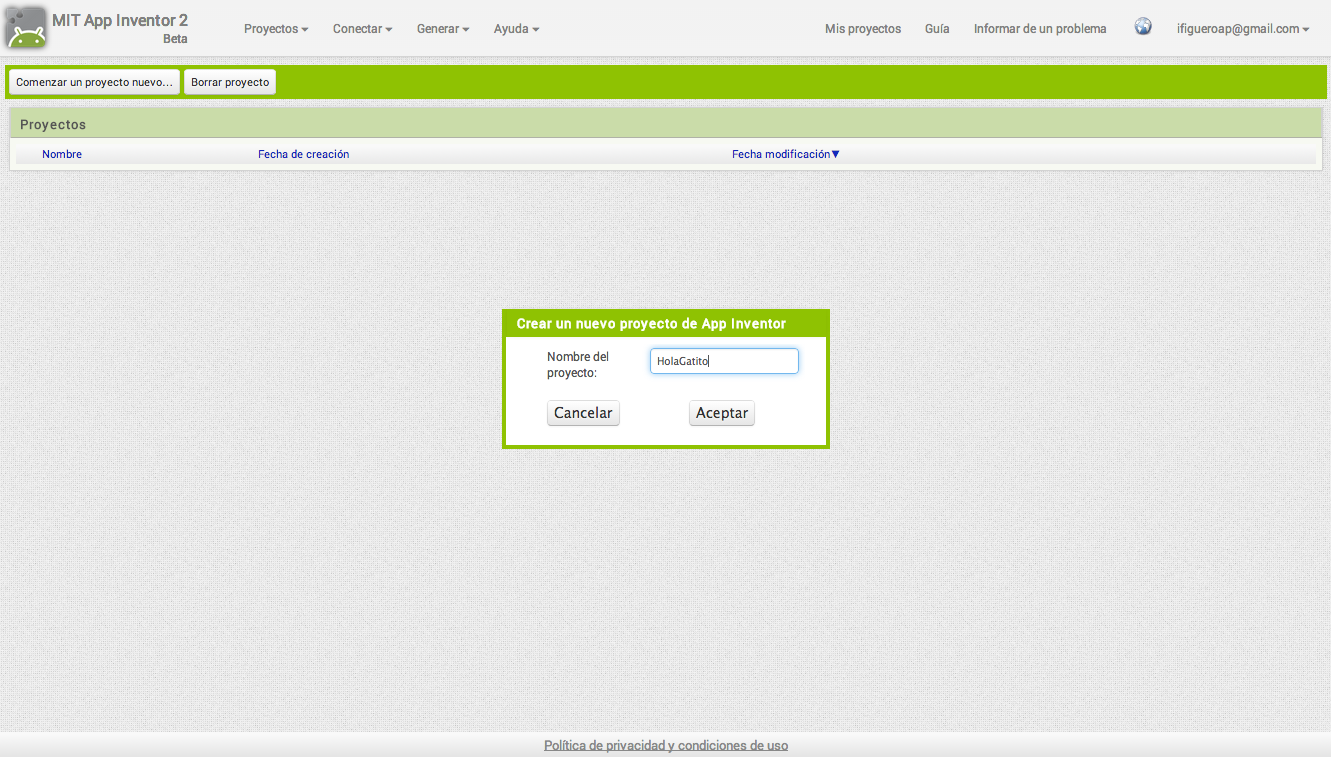
\includegraphics[scale=0.25]{CrearProyecto}
\caption{Crear proyecto \appName{Hola Gatito}}
\label{fig:crearProyecto}
\end{figure}

La primera ventana que se abre es el \componentDesigner. El \blockEditor está
disponible al hacer click en el botón ``Bloques'' en la esquina
superior derecha de la ventana.

\AppInventor es una herramienta computacional \emph{en la nube}, lo
que significa que tu aplicación está almacenada en un servidor en
línea mientras tú trabajas. Por lo tanto si cierras \AppInventor, tu
aplicación estará ahí cuando regreses; no necesitas guardar nada en tu
computador, como cuando trabajas con archivos de Word.

\subsection*{Diseñando los Componentes}

La primera herramienta que utilizarás es el \componentDesigner (o
simplemente \designer). Los componentes son los elementos que combinas
para crear aplicaciones, parecido a los ingredientes de una
receta. Algunos componentes son muy simples, como una
\component{Etiqueta}, la cual muestra texto en la pantalla, o un
\component{Botón}, el cual presionas para iniciar una acción. Otros
componentes son más elaborados: un \component{Lienzo} para dibujar,
que puede contener imágenes estáticas (sin movimiento) y también
animaciones; un \component{Acelerómetro}, que es un sensor de
movimiento que funciona de manera parecida a un Wiimote y detecta
cuando mueves o agitas el dispositivo. Otros componentes permiten
enviar y recibir mensajes de texto (SMS), reproducir música, sonidos,
videos, obtener información desde sitios web, etc.

Cuando abras el \designer, éste aparecerá como se muestra en
la~\Cref{fig:emptyDesigner}

\begin{figure}[H]
\centering
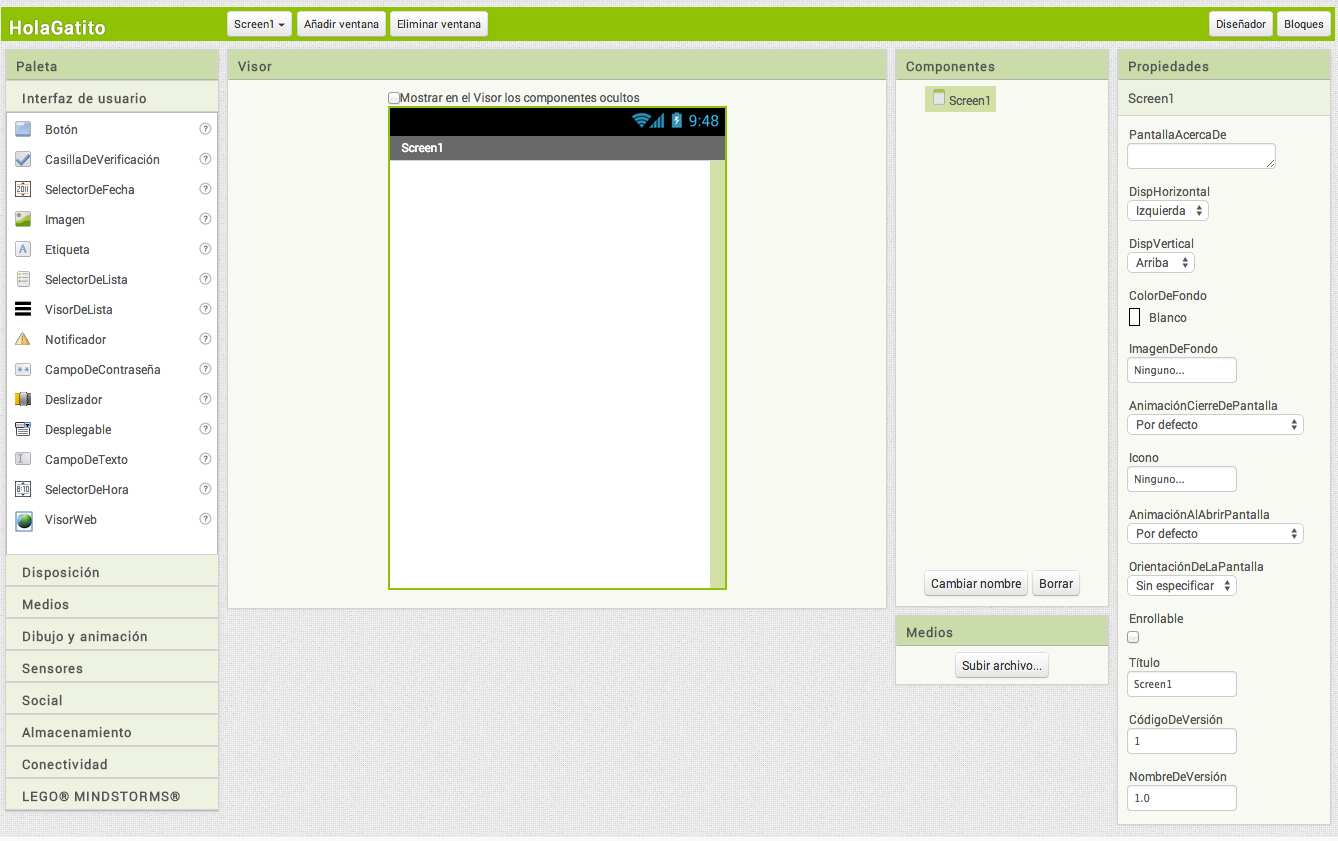
\includegraphics[scale=0.25]{emptyDesigner}
\caption{El \componentDesigner}
\label{fig:emptyDesigner}
\end{figure}

El \designer está dividido en varias áreas:

\begin{itemize}

\item En el centro hay un área que se llama \viewer. Aquí es donde tú
  colocas los componentes y los ordenas para especificar cómo quieres
  que se vea tu aplicación. El \viewer muestra una aproximación o
  borrador de cómo se verá la aplicación, por lo que, por ejemplo, una
  línea de texto podría cortarse en una posición distinta según el
  dispositivo que uses. Para ver \emph{realmente} cómo se verá una
  aplicación es necesario probarla directamente en un dispositivo.

\item A la izquierda del \viewer está la \palette, que es una lista de
  todos los componentes que puedes usar en tu aplicación. La \palette
  está dividida en secciones. Inicialmente sólo los componentes de la
  Interfaz de Usuario están visibles, pero basta con hacer click en
  los nombres de las otras secciones para ver los componentes de cada
  una de ellas (por ejemplo, Medios, Sensores, etc.).

\item A la derecha del \viewer está la lista de \componentList, que
  muestra los componentes usados en tu proyecto. Cualquier componente
  que arrastres en el \viewer también aparecerá en esta
  lista. Actualmente, el proyecto sólo tiene un componente:
  \component{Screen1}, que representa la pantalla del dispositivo.

\item Abajo del área \componentList se muestran los \media (imágenes y
  sonidos) en el proyecto. Este proyecto todavía no tiene ningún
  archivo multimedia, pero pronto agregarás algunos.

\end{itemize}

Al extremo derecho de la pantalla hay una sección que muestra las
\properties de los componentes; cuando seleccionas un componente en el
\viewer, verás su lista de \properties en esta sección. Las
\properties son detalles sobre cada componente que tú puedes
cambiar. Por ejemplo, al seleccionar una \component{Etiqueta}, puedes
ver propiedades relaconadas al color, texto, tipo de letra, etc. En
este momento está mostrando las propiedades de la pantalla, de nombre
\component{Screen1}, las que incluyen el color de fondo, imagen de
fondo y título, entre otras.

Para la aplicación \appName{Hola Gatito} necesitarás dos componentes
\emph{visibles} (puedes pensar sobre este tipo de componentes como
aquellos que se pueden ver en la aplicación): la \component{Etiqueta}
que muestra el texto ``Hola Gatito'' y un \component{Botón} con una
imagen de un gato. También necesitarás un componente de
\component{Sonido}, que es \emph{no-visible}, y que sabe cómo
reproducir sonidos, tales como el maullido del gato. Además,
necesitarás otro componente no-visible, el \component{Acelerómetro},
para detectar cuándo el dispositivo está siendo agitado. Ahora veremos
paso a paso cómo construir la aplicación con cada uno de estos
componentes.

\subsubsection*{Agregar la Etiqueta}

El primer componente por agregar es una \component{Etiqueta}:

\begin{enumerate}

\item Selecciona la sección ``Interfaz de Usuario'' en la \palette (si
  es que no está ya abierta), y arrastra una \component{Etiqueta}
  hacia el \viewer. Luego de hacerlo, verás una forma rectangular en
  el \viewer con el texto ``Texto para Etiqueta1''.

\item En el área de \properties de la etiqueta, busca la propiedad
  ``Texto''. Cambía el valor de esta propiedad por el texto ``Hola
  Gatito'' y luego presiona Enter. Verás que el texto cambia en el
  \viewer.

\item Cambia el \backgroundColor de la etiqueta haciendo click en la
  caja, que actualmente dice ``Ninguno'', para seleccionar un color de
  la lista que aparecerá. Selecciona Azul. También cambia el
  \textColor de la etiqueta a Amarillo. Finalmente, cambia el
  \fontSize a 20.

\end{enumerate}

Luego de seguir estos pasos, el \designer debería verse como en
la~\Cref{fig:holaGatitoStep1}.

\begin{figure}[H]
\centering
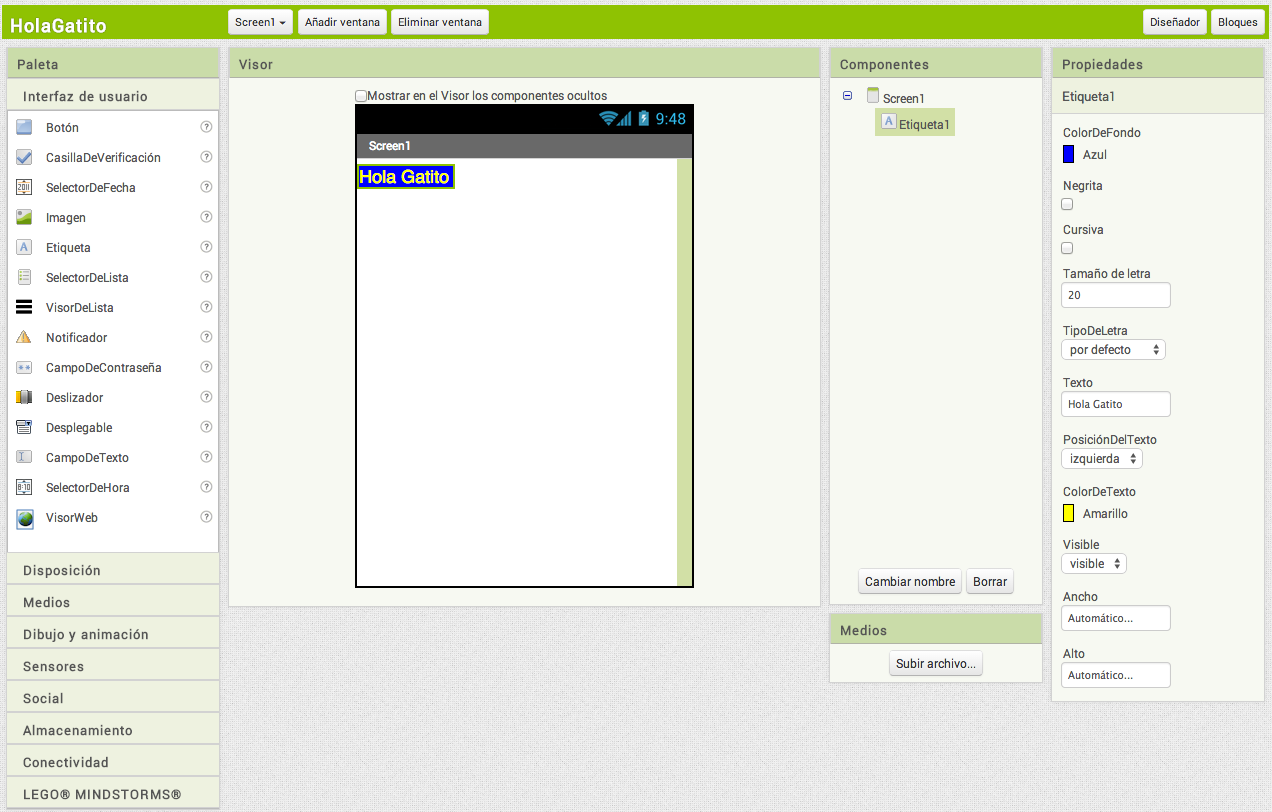
\includegraphics[scale=0.25]{holaGatitoStep1}
\caption{La aplicación ahora tiene una etiqueta}
\label{fig:holaGatitoStep1}
\end{figure}

\subsubsection*{Agregar el Bóton}
El gatito para \appName{Hola Gatito} está implementado como un
\component{Botón}---creas un botón normal, y luego cambias su imagen
de fondo a la del gatito. Para primero agregar un botón normal, debes
buscar el componente \component{Botón} en la \palette. Arrastra el
botón hacia el \viewer, ubicándolo debajo de la etiqueta. Verás que un
botón rectangular aparece en el \viewer.

Ahora tenemos un botón que usaremos para gatillar el efecto de sonido
cuando alguien lo presiona, pero lo que realmente queremos es ver la
foto de un gatito, y no un simple rectángulo. Para hacer que el botón
se vea como la foto del gatito debes hacer lo siguiente:

\begin{enumerate}

\item Primero, necesitas descargar una imagen del gatito y guardarla
  en tu computador. Puedes descargar la imagen disponible en
  \resources{ProgramaTusIdeas/Dia1/HolaGatito/gatito.png}. \emph{.png} es una
  extensión para un formato de archivo estándar, similar a \emph{.jpg}
  y \emph{.gif}; todos estos formatos pueden ser usados por
  \AppInventor, así como la mayoría de los formatos de sonido
  estándar, como \emph{.mpg} o \emph{.mp3}. También puedes descargar
  el sonido del maullido desde
  \resources{ProgramaTusIdeas/Dia1/HolaGatito/miau.mp3}. Si quieres, puedes usar
  tus propias imágenes y sonidos.

\item El área de \properties debería mostrar las propiedades del
  botón. Si no es así, selecciona el botón en el \viewer para que así
  sea. En las propiedades del botón presiona el área bajo el teto
  ``Imagen'' (que actualmente dice ``Ninguno'').

\item Presiona ``Subir archivo'', y luego presiona ``Seleccionar
  archivo'' para buscar en tu computador el archivo con la foto del
  gatito (si no usas tu propia imagen, el nombre es
  \mediafile{gatito.png}). Luego presiona ``Aceptar''.

\item Luego que la imagen se suba, el nombre de archivo debería estar
  disponible como una opción para la propiedad \property{Imagen} del
  botón. Presiona ``Aceptar'' para seleccionarla. También verás el
  archivo listado en el área de \media en la ventana del
  \designer. Además, en el \designer verás que el botón ahora se ve
  como la foto del gatito que acabas de seleccionar.

\item Quizás te diste cuenta que la foto del gatito todavía tiene las
  palabras ``Texto para Botón1''. Probablemente no quieras eso en tu
  aplicación, por lo tanto borra el texto de la propiedad
  \property{Texto} para el componente \component{Botón1}.

\end{enumerate}

Ahora el \designer debería verse como en
la~\Cref{fig:holaGatitoStep2}.

\begin{figure}[H]
\centering
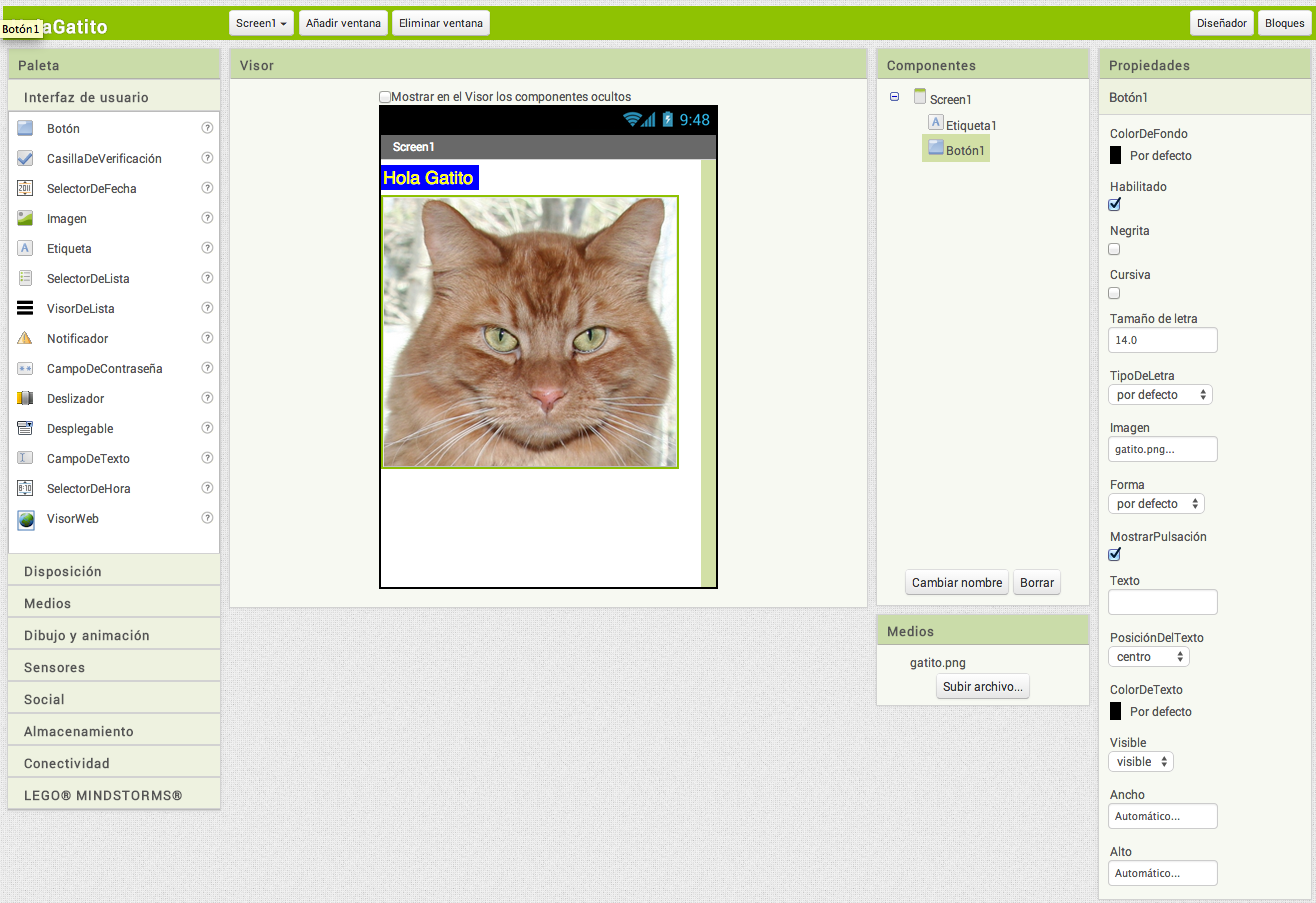
\includegraphics[scale=0.25]{holaGatitoStep2}
\caption{La aplicación con una etiqueta y un botón con una imagen de
  un gatito}
\label{fig:holaGatitoStep2}
\end{figure}

\subsubsection*{Agregar el Maullido}

En tu aplicación quieres que el gatito maulle cuando el botón sea
presionado. Para esto, necesitarás agregar el sonido del maullido, y
programar el comportamiento del botón para reproducir ese sonido
cuando el botón es presionado:

\begin{enumerate}

\item Si aún no has descargado el sonido del maullido, descárgalo
  ahora desde \resources{ProgramaTusIdeas/Dia1/HolaGatito/miau.mp3}.

\item Ve a la \palette, y selecciona la sección \media. Arrastra un
  componente \component{Sonido} y cólocalo en el \viewer. Sin importar
  el lugar donde lo arrastraste, este componente aparecerá en un área
  abajo del \viewer, llamada ``Componentes no visibles''. Los
  componentes no visibles son objetos que hacen cosas para la
  aplicación pero que no aparecen en la interfaz visual del usuario de
  la aplicación.

\item Selecciona el componente \component{Sonido1} para mostrar sus
  propiedades. Selecciona su propiedad \property{Origen} y sigue los
  pasos para subir el archivo \mediafile{miau.mp3} que descargaste
  anteriormente. Una vez que finalices este paso, deberías ver los
  archivos \mediafile{gatito.png} y \mediafile{miau.mp3} en el área de
  \media en el \designer.

\end{enumerate}

La tabla~FOO muestra los componentes que has agregado hasta ahora a la
aplicación \appName{Hola Gatito}.

\begin{footnotesize}
\begin{table}[H]
\centering
\begin{tabular}{|c|c|c|c|}
\hline
\textbf{Tipo de  Componente} & \textbf{Sección en la \palette} & \textbf{Nombre} & \textbf{Propósito}\\
\hline
Botón & Interfaz de usuario & Botón1 & Presionar para que el gato
maulle.\\
\hline
Etiqueta & Interfaz de usuario & Etiqueta1 & Muestra el texto ``Hola
Gatito''.\\
\hline
Sonido & Medios & Sonido1 & Reproduce el sonido del maullido.\\
\hline
\end{tabular}
\caption{Componentes que has agregado a la aplicación \appName{Hola Gatito}}
\label{tab:holaGatitoComponents}
\end{table}
\end{footnotesize}

\subsection*{Probar la Aplicación}

Con \AppInventor, puedes ver y probar tu aplicación en un dispositivo
Android a medida que la vas creando. Probar tu aplicación de manera
incremental, paso a paso mientras la desarrollas, es una práctica
usada por muchos desarrolladores de software, y que te ahorrará muchas
horas de trabajo!

\paragraph{Conexión por puerto USB}
Para conectar las aplicaciones de \AppInventor con tus dispositivos
Android usaremos una conexión por cable USB. Esto requiere la
instalación de un software especial en tu computador---pero que ya
está preinstalado!\footnote{Las instrucciones de instalación, en
  inglés, están disponibles en
  \url{http://appinventor.mit.edu/explore/ai2/setup.html}}

Para probar tu aplicación, conecta tu dispositivo al computador usando
un cable USB, y luego selecciona la opción ``Conectar'' y
específicamente la opción ``USB'', tal como se muestra en la~\Cref{fig:conectarUSB}

\begin{figure}[H]
\centering
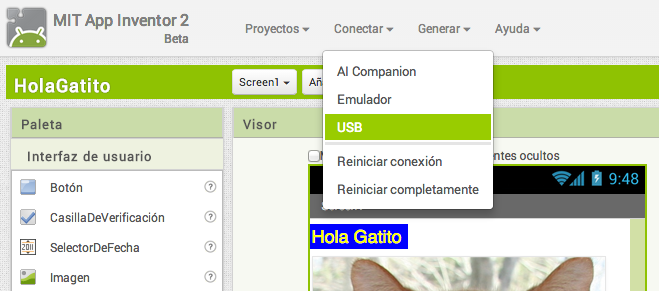
\includegraphics[scale=0.25]{ConectarUSB}
\caption{Conexión \AppInventor por USB}
\label{fig:conectarUSB}
\end{figure}

Si todo funciona correctamente, deberías ver la aplicación
\appName{Hola Gatito} ejecutándose en tu dispositivo, incluyendo todos
los componentes que agregaste. A medida que hagas cambios en el
\componentDesigner o en el \blockEditor, estos cambios también
aparecerán en el dispositivo. Consulta a tu tutor ante cualquier
problema.

Si tu aplicación aparece en el dispositivo, presiona la imagen del
gato. ¿Crees que algo pasará? En realidad no pasará nada, porque tu
aplicación todavía no le ha dicho al botón qué es lo que debe hacer al
ser presionado. Este es el primer punto importante para comprender
sobre \AppInventor: para cada componente que agregas en el \designer,
tienes que ir hacia el \blockEditor y crear el código para que algo
pase con ese componente.

\subsection*{Agregando Comportamiento a los Componentes}

Acabas de agregar componentes de tipo \component{Botón},
\component{Etiqueta} y \component{Sonido} como los bloques con los que
construyes tu primera aplicación. Ahora hagamos que el gatito maulle
cuando presionas el botón. Esto tienes que hacerlo con el
\blockEditor. Presiona el botón ``Bloques'' en la esquina superior
derecha del \componentDesigner.

Observa bien la ventana del \blockEditor. Aquí es donde le dices a los
componentes qué hacer y cómo hacerlo. Ahora le dirás al botón del
gatito que reproduzca un sonido cuando el usuario lo presiona. Si los
componentes son los ingredientes en una receta, puedes pensar que los
bloques son las instrucciones de cocina.

\subsubsection*{Haciendo Maullar al Gatito}

En la esquina superior izquierda de la ventana, debajo del encabezado
``Bloques'', puedes ver una columna que incluye una sección
``Integrados'', y una sección para cada componente de los que creaste
en el \designer: \component{Botón1}, \component{Etiqueta1}, y
\component{Sonido1}. Cuando haces click en uno de los componentes,
aparecen un montón de opciones (bloques) para ese componente. Presiona
el componente \component{Botón1}. Al hacerlo, se muestra una selección
de los bloques que puedes usar para decirle al botón qué debe hacer;
esta lista comienza con el bloque \block{Botón1.Click}, como se
muestra en la~\Cref{fig:button1Blocks}.

\begin{figure}[H]
\centering
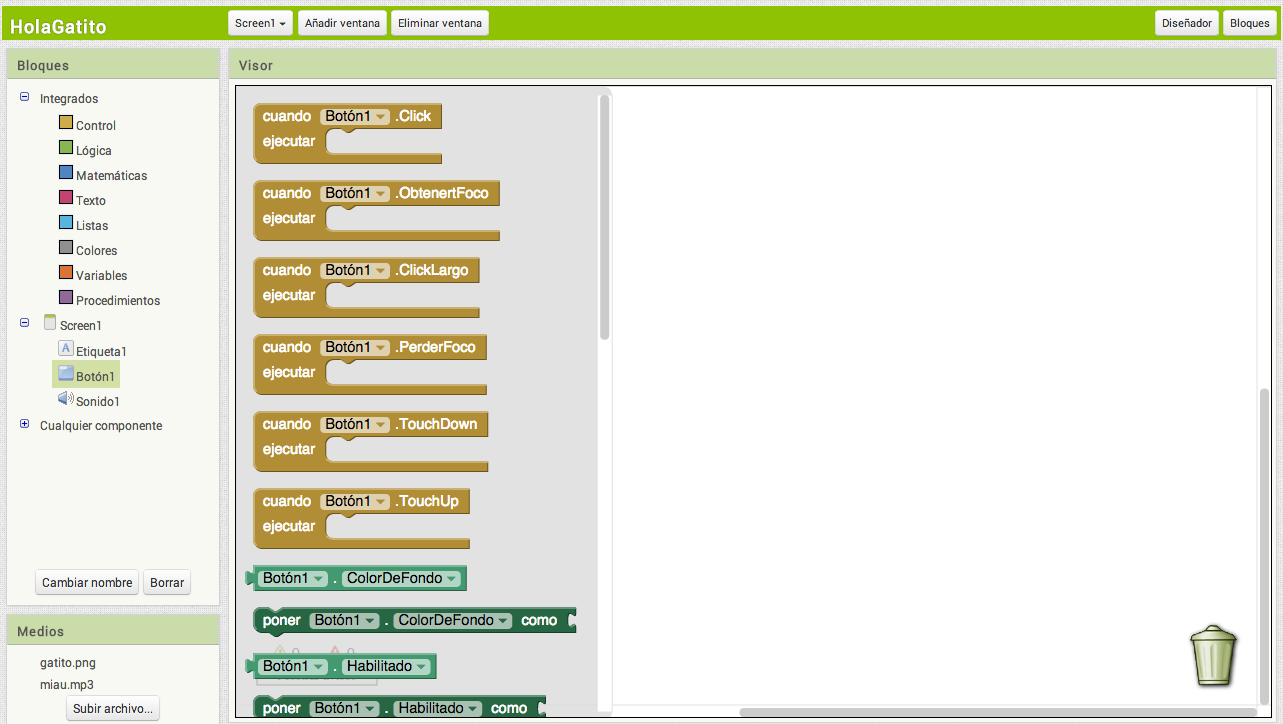
\includegraphics[scale=0.25]{button1Blocks}
\caption{Al seleccionar el componente \component{Botón1} se muestran
  sus bloques}
\label{fig:button1Blocks}
\end{figure}

Arrastra el bloque \block{Botón1.Click} y arrástralo en el \viewer (el
espacio en blanco para trabajar con los bloques). Puedes darte cuenta
que la palabra \emph{cuando} está incluida en el bloque. Los bloques
que incluyen la palabra \emph{cuando} se llaman \emph{controladores de
  eventos}. Ellos especifican lo que los componentes deberían hacer
\emph{cuando} algun evento particular ocurre. En este caso, estamos
interesados en el evento de que un usuario de la aplicación presione
el gatito (que en realidad es un botón), tal como se muestra en
la~\Cref{fig:button1ClickEmpty}. Luego, agregaremos algunos bloques
para programar lo que pasará en respuesta a ese evento.

\begin{figure}[H]
\centering
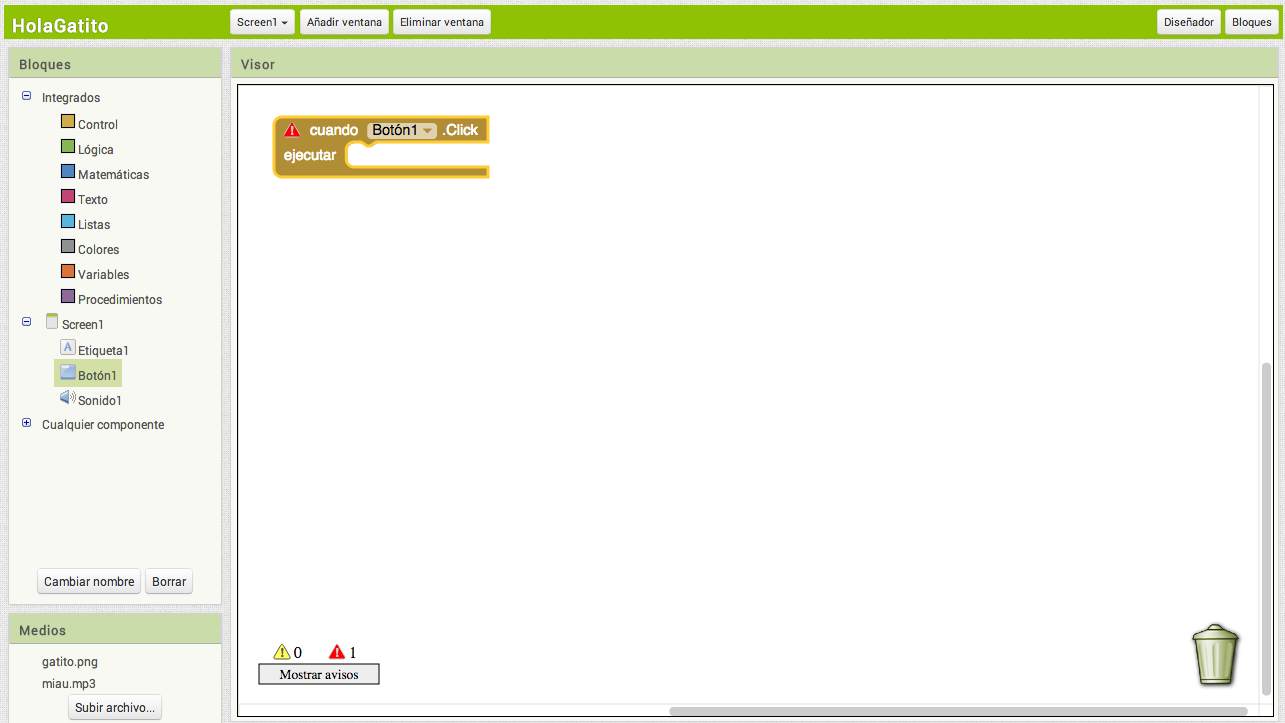
\includegraphics[scale=0.25]{button1ClickEmpty}
\caption{Especificarás una respuesta al usuario que presiona el botón
  usando el bloque \block{Boton.Click}}
\label{fig:button1ClickEmpty}
\end{figure}

Ahora selecciona el componente \component{Sound1} y luego arrastra el
bloque \block{llamar Sonido1.Reproducir}. Recuerda que anteriormente
configuramos el \property{Origen} del componente con el archivo
\mediafile{miau.mp3}. Observa ahora que el bloque \block{llamar
  Sonido1.Reproducir} tiene una forma tal que es posible ensamblarlo
con el espacio marcado como ``ejecutar'' en el bloque
\block{Botón1.Click}. \AppInventor está diseñado de manera que sólo
ciertos bloques pueden ser ensamblados juntos; de esta manera tu
siempre sabrás que estás conectando bloques que en realidad trabajan
juntos. En este caso, los bloques con la palabra \emph{llamar} hacen
que los componentes hagan cosas. Los dos bloques deben conectarse para
formar una sola unidad, como se muestra en
la~\Cref{fig:button1ClickPlay}. Escucharás un sonido cuando los
bloques se conecten correctamente.

\begin{figure}[H]
\centering
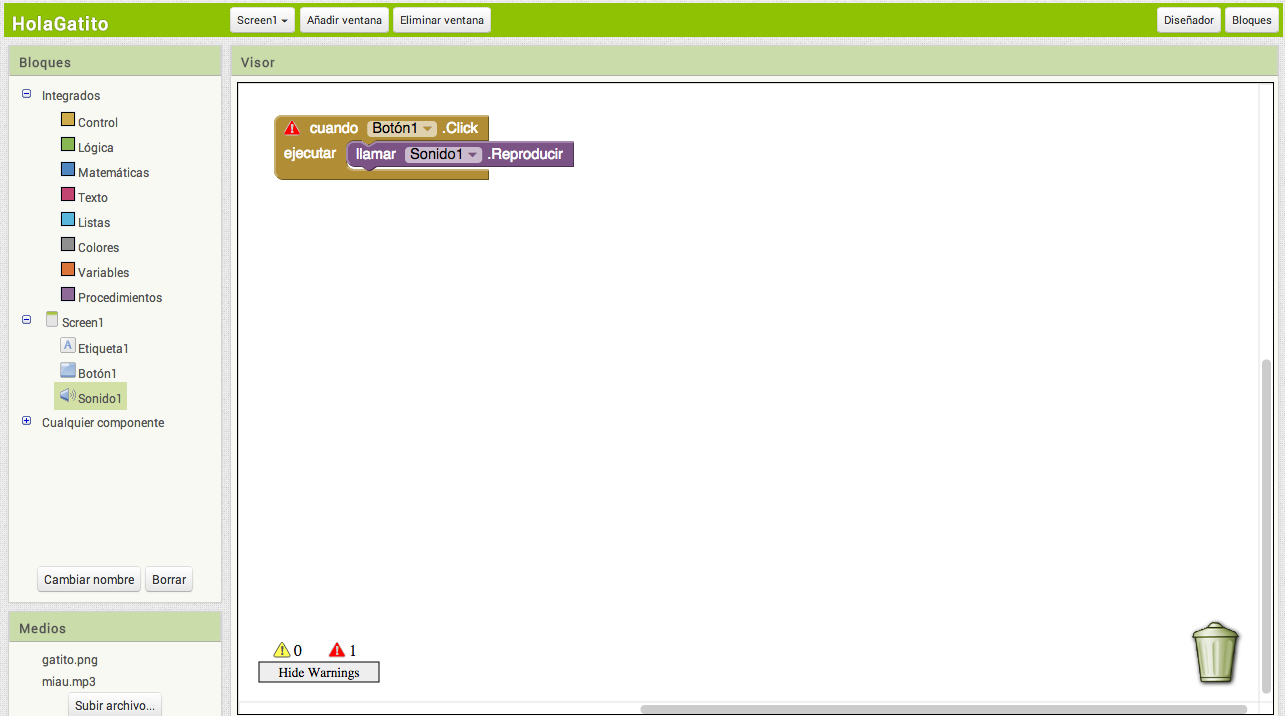
\includegraphics[scale=0.25]{button1ClickPlay}
\caption{Ahora cuando alguien presione el botón, se escuchará el maullido}
\label{fig:button1ClickPlay}
\end{figure}

A diferencia del código programado de manera tradicional (el que a
menudo se ve como un revoltijo de ``jerigonza''), los bloques de
eventos-respuestas en \AppInventor describen los comportamientos que
estás intentando crear. En este caso, estamos esencialmente diciendo
``Oye \AppInventor, cuando alguien presione el botón del gatito,
reproduce el sonido del maullido''.

\paragraph{Prueba tu Aplicación} Asegúrate que todo esté funcionando
correctamente---es importante que pruebes tu aplicación cada vez que
agregas algo nuevo. Presiona el botón en el dispositivo. Deberías
escuchar el maullido. Felicitaciones, tu primera aplicación se está
ejecutando!

\subsubsection*{Agregar el Ronrroneo}
Ahora vamos a hacer que el gato ronrronee y maulle cuando presionas el
botón. Simularemos el ronrroneo haciendo vibrar el dispositivo. Eso
puede sonar difícil, pero en realidad es muy fácil porque el
componente \component{Sonido} que usamos para reproducir el maullido
también puede hacer vibrar el dispositivo. \AppInventor te ayuda a
aprovechar la funcionalidad esencial de los dispositivos sin tener que
preocuparse de \emph{cómo} el dispositivo vibra en la práctica. No
necesitas hacer nada nuevo en el \designer, simplemente puedes agregar
un nuevo comportamiento al botón en el \blockEditor.

\begin{enumerate}

\item Ve al \blockEditor y selecciona el componente
  \component{Sonido1}.

\item Selecciona el bloque \block{llamar Sonido1.Vibrar} y arrastralo
  hacia abajo del bloque \block{llamar Sonido1.Reproducir}. El bloque
  debería ajustarse en su lugar, como se muestra en
  la~\Cref{fig:button1ClickPlayVibrate}.

\begin{figure}[H]
\centering
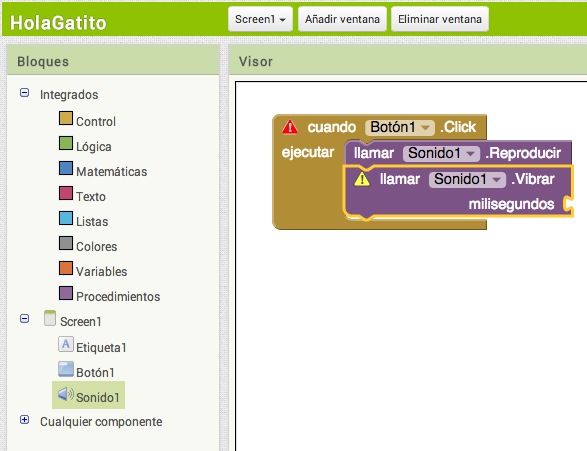
\includegraphics[scale=0.25]{button1ClickPlayVibrate}
\caption{Reproduciendo el sonido y vibrando en el evento Click}
\label{fig:button1ClickPlayVibrate}
\end{figure}


\item Observa ahora que el bloque \block{llamar Sonido1.Vibrar}
  incluye el texto ``milisegundos''. Un espacio abierto en un bloque
  significa que necesitas conectar algo ahí para especificar en
  detalle el comportamiento del bloque. En este caso, debes decirle al
  bloque por cuánto tiempo debería vibrar. Necesitas agregar esta
  información en milésimas de segundo (milisegundos), lo que es
  bastante común en muchos lenguajes de programación. Por lo tanto,
  para hacer que el dispositivo vibre por medio segundo, tienes que
  poner un valor de 500 milisegundos. Para poner un valor de 500
  necesitas arrastrar un bloque numérico. Selecciona el componente
  integrado ``Matemáticas'', como se muestra en
  la~\Cref{fig:button1ClickPlayVibrateMillis}. Deberías ver un bloque
  con un cero como primer elemento. Puedes arrastrar este bloque y
  cambiar su valor por cualquier otro número.

\begin{figure}[H]
\centering
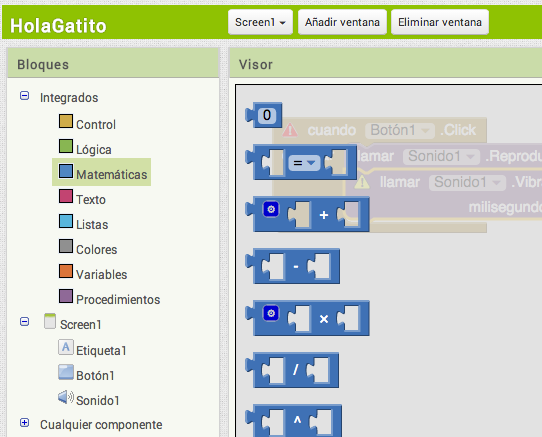
\includegraphics[scale=0.25]{button1ClickPlayVibrateMillis}
\caption{Agregando un bloque numérico para especificar la duración de
  la vibración}
\label{fig:button1ClickPlayVibrateMillis}
\end{figure}

\item Arrastra el bloque numérico y verás un bloque azul con el número
  cero, como se muestra en
  la~\Cref{fig:button1ClickPlayVibrateMillis2}.

\begin{figure}[H]
\centering
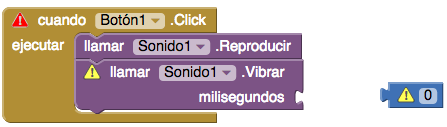
\includegraphics[scale=0.25]{button1ClickPlayVibrateMillis2}
\caption{Agregando un bloque numérico (0 es el valor por defecto).}
\label{fig:button1ClickPlayVibrateMillis2}
\end{figure}

\item Cambia el 0 a 500 haciendo click en el bloque y escribiendo el
  nuevo valor, como se muestra en
  la~\Cref{fig:button1ClickPlayVibrateMillis3}.

\begin{figure}[H]
\centering
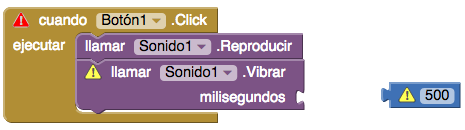
\includegraphics[scale=0.25]{button1ClickPlayVibrateMillis3}
\caption{Cambiando el valor del bloque numérico a 500.}
\label{fig:button1ClickPlayVibrateMillis3}
\end{figure}

\item Conecta el bloque numérico 500 en el espacio del bloque
  \block{llamar Sonido1.Vibrar}, como se muestra en
  la~\Cref{fig:button1ClickPlayVibrateMillis4}

\begin{figure}[H]
\centering
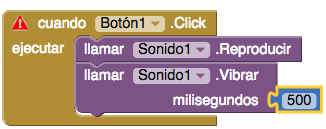
\includegraphics[scale=0.25]{button1ClickPlayVibrateMillis4}
\caption{Conectando el bloque numérico 500 en el espacio para
  configurar los milisegundos.}
\label{fig:button1ClickPlayVibrateMillis4}
\end{figure}

\end{enumerate}

\paragraph{Prueba tu aplicacion!}

\subsubsection*{Agitando el Dispositivo}

Ahora agreguemos un elemento final que aprovecha otra característica
de Android: hacer que el gatito maulle cuando agitas el
dispositivo. Para hacer esto, usarás un componente llamado
\component{Acelerómetro} que puede sentir cuando agitas o mueves el
dispositivo.

\begin{enumerate}

\item En el \designer, expande la sección \sensors en la \palette y
  arrastra un \component{Acelerómetro} hacia el \viewer. No te
  preocupes sobre el lugar donde lo arrastrarás, ya que es un
  componente no visible que aparecerá en la sección justo abajo del
  \viewer.

\item Vas a querer manejar el que alguien agite el dispositivo como un
  evento diferente y separado de cuando se presiona el botón. Eso
  significa que necesitas un nuevo controlador de eventos. Ve al
  \blockEditor, donde debería haber un nuevo componente
  \component{Acelerómetro1}. Seleccionalo y arrastra el bloque
  \block{Acelerómetro1.Agitar}.

\item De la misma forma que lo hiciste con el botón cuando es
  presionado, arrastra un bloque \block{llamar Sonido1.Reproducir} y
  conéctalo en el espacio del bloque \block{Acelerómetro1.Agitar}. Los
  bloques de la aplicación deben quedar como los que se muestran en
  la~\Cref{fig:holaGatitoBlocks}. Prueba tu aplicación agitando el
  dispositivo!

\begin{figure}[H]
\centering
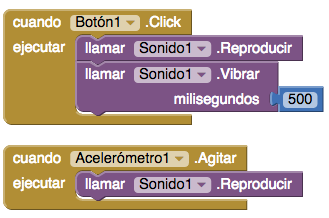
\includegraphics[scale=0.25]{holaGatitoBlocks}
\caption{Los bloques para la aplicación \appName{Hola Gatito}}
\label{fig:holaGatitoBlocks}
\end{figure}

\end{enumerate}

\subsection*{Compartir tu Aplicación}

Puedes compartir tu aplicación de varias maneras. Para compartir la
aplicación ejecutable (el archivo .apk que se instala directamente en
un dispositivo), primero presiona ``Generar'' y escoge ``App (guardar
archivo .apk en mi ordenador''. Esto creará un archivo con una
extensión \emph{.apk} en tu computador. Puedes compartir este archivo
con otros envíandolo como archivo adjunto en un correo, el cual
abrirán con su cliente de correo en el dispositivo donde instalarán la
aplicación. También puedes subir el archivo .apk en la web (por
ejemplo en DropBox o en tu portafolio). Sólo debes asegurarte que las
personas que quieran instalar tu aplicación deben permitir las
``fuentes desconocidas'' en la configuración del dispositivo, para
permitir la instalación de aplicaciones que no provienen de la tienda
de aplicaciones de Android.

También puedes crear un código QR para tu aplicación de manera que las
personas puedan escanear el código en sus dispositivos, desde la web o
incluso desde algún poster. Existen numerosas herramientas para crear
un código QR desde una URL (por ejemplo,
\url{http://qrcode.kaywa.com/}). Una vez que tengas el código QR
puedes insertarlo en una página web u otros documentos.

Además, también puedes compartir el \emph{código fuente} (los bloques)
de tu aplicación con otro desarrollador que use \AppInventor. Para
hacer esto, selecciona ``Mis Proyectos'', elige la aplicación que
deseas compartir (en este caso \appName{HolaGatito}), selecciona
``Proyecto'', y luego selecciona ``Exportar a mi ordenador el proyecto
(.aia) seleccionado''. El archivo creado en tu computador tendrá
extensión \emph{.aia}. Esto le dará a otra persona una copia completa
de tu aplicación, la que podrán usar para editar y personalizar sin
afectar tu propia versión.

\subsection*{Personalizaciones}

Después que desarrolles las aplicaciones de este taller, seguramente
pensarás muchas maneras de mejorarlas. A medida que avancemos con las
aplicaciones, también te sugeriremos ideas para que intentes
implementarlas. El personalizar las aplicaciones te llevará a explorar
los componentes y bloques disponibles, y a aprender a programar por ti
mismo sin las instrucciones detalladas que son dadas en los
tutoriales. 

Aquí hay algunas ideas para mejorar la aplicación \appName{Hola
  Gatito}:

\begin{itemize}

\item Mientras agitas el dispositivo, los maullidos sonarán de forma
  extraña, como si hubiera eco. Esto pasa porque el acelerómetro está
  gatillando el evento agitar muchas veces por segundo, por lo que los
  maullidos se solapan. Si te fijas en el componente
  \component{Sonido} en el \designer, verás una propiedad que se llama
  \property{IntervaloMinimo}. Esta propiedad determina el tiempo
  mínimo que hay que esperar para reproducir dos sonidos de forma
  consecutiva. Actualmente tiene un valor de 400 milisegundos (casi
  medio segundo), lo que es menor que la duración de un
  maullido. Jugando con el valor de esta propiedad podrás cambiar la
  manera en que los maullidos se solapan entre sí.

\item Si exportas la aplicación, la ejecutas, y luego caminas con tu
  dispositivo en el bolsillo, tu dispositivo maullará cada vez que te
  muevas bruscamente---algo que quizás pueda ser vergonzoso! Las
  aplicaciones Android típicamente están diseñadas para seguir
  ejecutándose incluso cuando no las estas mirando; por lo que tu
  aplicación sigue comunicándose con el acelerómetro y los maullidos
  continúan. Para salir realmente de la aplicación, debes mantener
  presionado el botón de menu en la aplicación \appName{Hola
    Gatito}. Se te mostrará una opción para cerrar la aplicación, al
  seleccionarla la aplicación estará completamente cerrada.

\subsection*{Resumen}

A continuación repasamos los principales conceptos cubiertos en este
tutorial:

\begin{itemize}

\item Construyes aplicaciones seleccionando componentes en el
  \designer y diciéndoles qué hacer y cuándo hacerlo en el \blockEditor.

\item Algunos componentes son visibles y otros no lo son. Los visibles
  aparecen en la interfaz de usuario de la aplicación. Los no visibles
  hacen cosas como reproducir sonidos.

\item Defines el comportamiento de los componentes juntando bloques en
  el \blockEditor. Primero arrastras un controlador de eventos como
  \block{Boton1.Click}, y luego pones bloques de comandos como
  \block{Sonido1.Reproducir} en su interior. Cualquier bloque
  contenido dentro de \block{Boton1.Click} será realizado cuando el
  usuario presione el botón.

\item Algunos comandos necesitan información extra para hacerlos
  funcionar. Un ejemplo es \block{Sonido1.Vibrar}, que necesita saber
  cuántos milisegundos debe vibrar. Estos valores se llaman
  \emph{argumentos} o \emph{parámetros}.

\item Los números se representan como bloques numéricos. Puedes
  conectar estos bloques en comandos que toman números como
  argumentos.

\item \AppInventor tiene componentes que representan los sensores del
  dispositivo. El \component{Acelerómetro} puede detectar cuándo el
  dispositivo se mueve.

\item Puedes empaquetar las aplicaciones y descargarlas al teléfono,
  donde se ejecutan de forma independiente a \AppInventor.

\end{itemize}

\end{itemize}

\section{Discusión y Personalización}
\label{sec:disc-y-pers}

Para ayudarte a consolidar tus conocimientos sobre \AppInventor te
invitamos a responder las siguientes preguntas, y a personalizar tu
aplicación siguiendo las sugerencias que se presentan a continuación.

\paragraph{Preguntas}

\begin{enumerate}

\item \AppInventor tiene dos ventanas principales. ¿Cuáles son y qué
  haces en ellas?

\item Probando e Instalando una Aplicación

  \begin{itemize}

  \item ¿Cómo pruebas una aplicación a medida que la vas desarrollando?

  \item ¿Cómo puedes instalar una aplicación, que tú construiste, en
    tu dispositivo Android?

  \item ¿Qué pasaría si no tuvieras un teléfono o tablet, pero
    quisieras programar algunas aplicaciones? ¿Podrías hacerlo? ¿Cómo
    lo harías?

  \end{itemize}

\item En la aplicación \appName{Hola Gatito} menciona un(a):

  \begin{itemize}
  
  \item componente visible

  \item componente no visible

  \item propiedad

  \item evento

  \item controlador de eventos

  \item llamada a función

  \end{itemize}

\item ¿Qué es un controlador de eventos? ¿De qué está compuesto?

\item Una aplicación consiste de su interfaz de usuario y su
  comportamiento. ¿En qué consiste el comportamiento de la aplicación?

\end{enumerate}

\paragraph{Ejercicios de Personalización}

\begin{enumerate}

\item Agrega un componente \component{CasillaDeVerificación} que
  indica si el gatito está durmiendo o no. Si la casilla está
  chequeada, el gatito duerme, y si no, está despierto.

\item Modifica el comportamiento de la aplicación para tomar en cuenta
  si el gatito duerme o no. Mientras el gatito duerme, el presionar el
  botón no emite ningún sonido ni hace vibrar el dispositivo. Si el
  gatito duerme y se agita el dispositivo, entonces se despierta.

\end{enumerate}


\section{Creando tu Portafolio}
\label{sec:creando-tu-port}

En este tutorial te mostraremos cómo crear tu Portafolio, que incluirá
todo el trabajo que realices en el taller. Aprenderás a crear una
página en Google Sites, y a partir de este día deberás registrar todo
tu trabajo en este portafolio. ¿Por qué vale la pena tener un
portafolio? Algunas razones:

\begin{itemize}
\item Estarás creando sobre lo que tus compañeros y amigos pueden aprender.

\item Podrás continuar trabajando en tus proyectos después de que el
  taller termine.

\item Al tener todo tu trabajo en el portafolio puedes volver a
  proyectos anteriores a medida que progresas en el taller.

\item Puedes mostrar tu trabajo y progreso a tu familia, tus amigos,
  que podrán instalar las aplicaciones en sus dispositivos Android.

\item Google Sites es una herramienta que te puede ser útil en el futuro.
\end{itemize}

\paragraph{Google Sites: Tu sitio en la Nube} Utilizamos Google Sites
principalmente por las siguientes razones:

\begin{itemize}
\item WYSIWYG (What You See is What You Get): no necesitas saber HTML
  para editar el sitio.

\item Colaborativo: puedes definir quién edita las páginas. Puedes ser
  sólo tu, o un grupo, o todo el mundo (como en la Wikipedia).

\item Está almacenado en la Nube: en los servidores de Google. Es
  difícil que se pierda tu información!

\item Puedes crear un sitio de manera instantánea y crear tantos como
  quieras, gratis.

\item No necesitas descargar o instalar ningún software en tu
  computador para modificar tus sitios.
\end{itemize}

\subsection*{Instrucciones}

\begin{enumerate}

\item Para usar Google Sites (y también \AppInventor) necesitas una
  cuenta de Google. Una vez que tengas la cuenta, abre en tu navegador
  web la página \url{http://sites.google.com}. Puedes ajustar las
  preferencias para que el sitio aparezca en Español.

\item Crea un nuevo sitio:

  \begin{itemize}
  \item Presiona el botón ``Crear''.
  \item Ingresa el nombre del sitio, algo como ``Mi Sitio de App
    Inventor''.
  \item Ajusta o ingresa la ubicación del sitio. Este nombre debe ser
    único, por lo que puede ocurrir que el nombre que querías ya esté
    ocupado. 
  \item Escoge la plantilla en blanco. Luego cuando tengas más tiempo
    puedes cambiar la plantilla y el diseño de tu sitio. Escribe el
    código de comprobación y luego presiona el botón
    ``Crear''. La~\Cref{fig:createSite} muestra la interfaz para crear
    el sitio.

\begin{figure}[H]
\centering
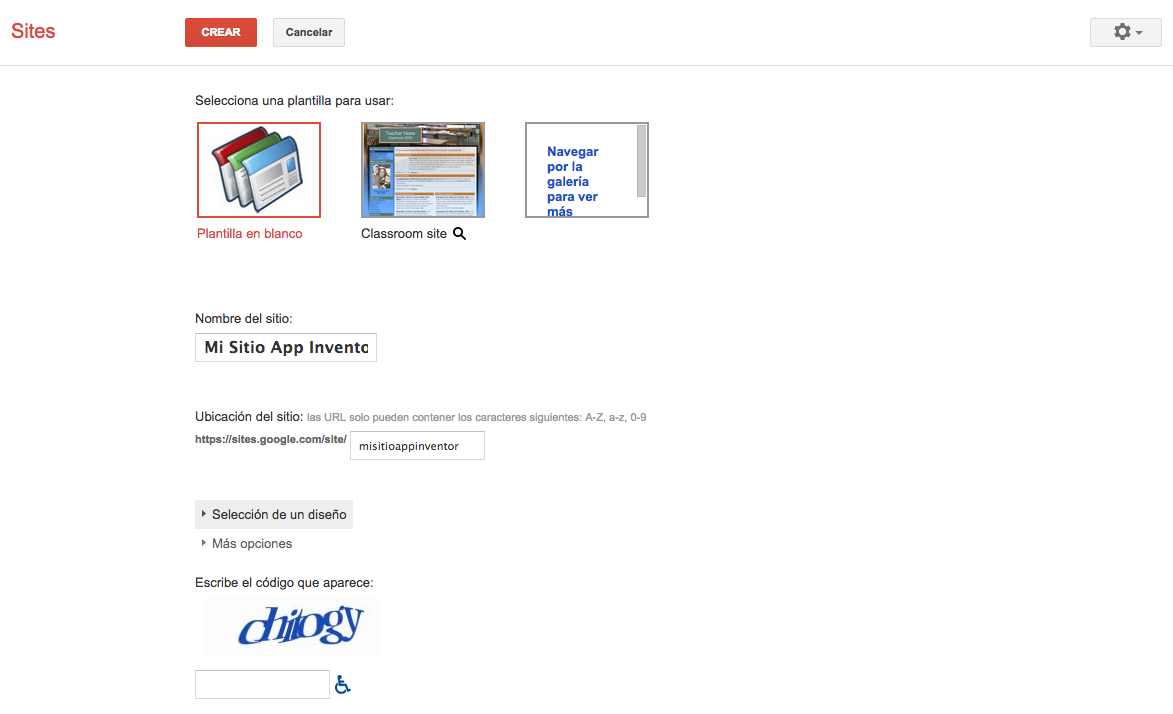
\includegraphics[scale=0.25]{CreateSite}
\caption{Datos necesarios para crear tu Portafolio en Google Sites.}
\label{fig:createSite}
\end{figure}
    
  \end{itemize}

\item Agrega alguna información básica a la página principal, como se
  muestra en la~\Cref{fig:SiteAddInfo}. Para editar la página presiona
  el botón ``Editar página'', que tiene el ícono de un lápiz, en la
  esquina superior derecha. Cuando estes en modo de edición, en la
  misma esquina aparecerán los botones ``Guardar'' y
  ``Cancelar''. Agrega información tal como:

  \begin{itemize}
  \item nombre e información de contacto
  \item una breve biografía
  \item algún comentario sobre el taller
  \end{itemize}

\begin{figure}[H]
\centering
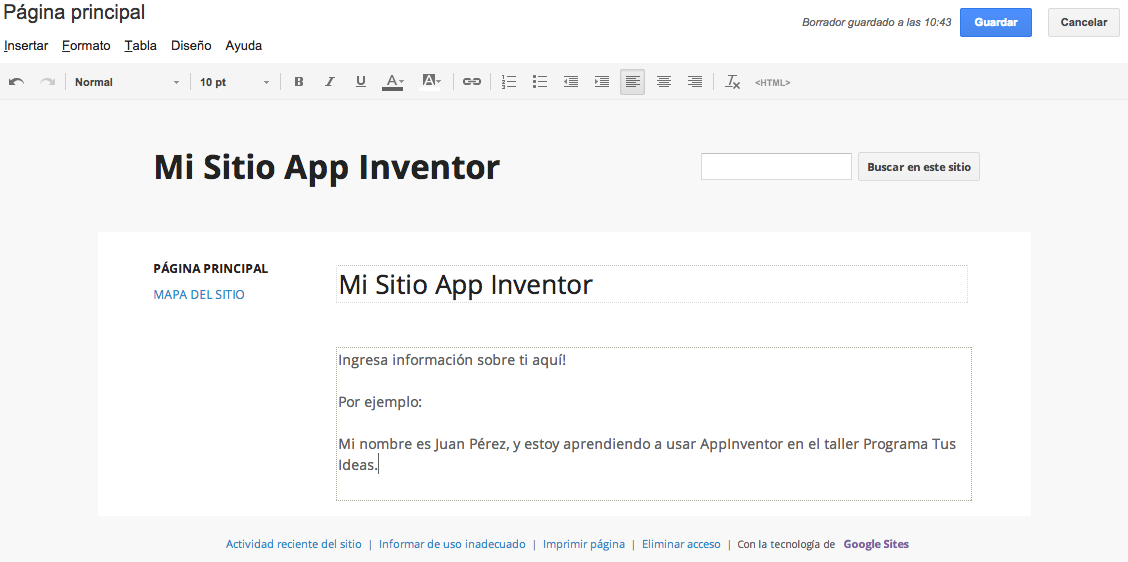
\includegraphics[scale=0.25]{SiteAddInfo}
\caption{Agregando información básica a tu Portafolio}
\label{fig:SiteAddInfo}
\end{figure}

\item Agrega una imagen de perfil a tu página principal. Puedes
  insertar imágenes ya sea desde tu computador, o desde la
  Web. Primero inserta una imagen desde la web. Abre otra ventana en
  tu navegador y busca en Google alguna imagen que quieras usar (ir a
  \url{http://images.google.com} para buscar imágenes). Cuando
  encuentras una imagen que te guste, presiona el botón derecho de tu
  mouse y selecciona la opción ``Copiar URL de imagen'', que pondrá la
  dirección en el portapapeles. La~\Cref{fig:SiteAddImage2} muestra
  cómo hacer esto.

\begin{figure}[H]
\centering
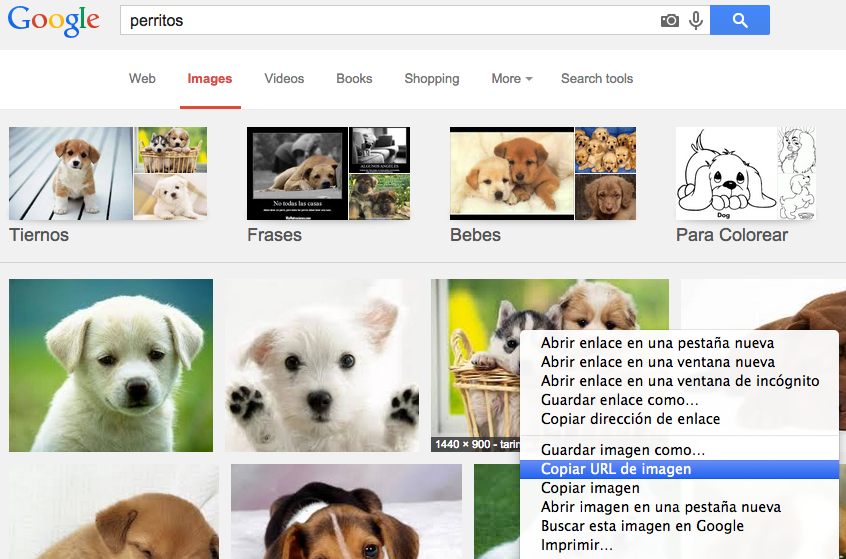
\includegraphics[scale=0.25]{SiteAddImage2}
\caption{Agregar una imagen desde la web, copiando su URL}
\label{fig:SiteAddImage2}
\end{figure}

\item Para poner la imagen en tu sitio, asegúrate de estar en modo de
  edición y selecciona la opción ``Insertar | Imagen'' en el menú,
  como se muestra en la~\Cref{fig:SiteAddImage1}.

\begin{figure}[H]
\centering
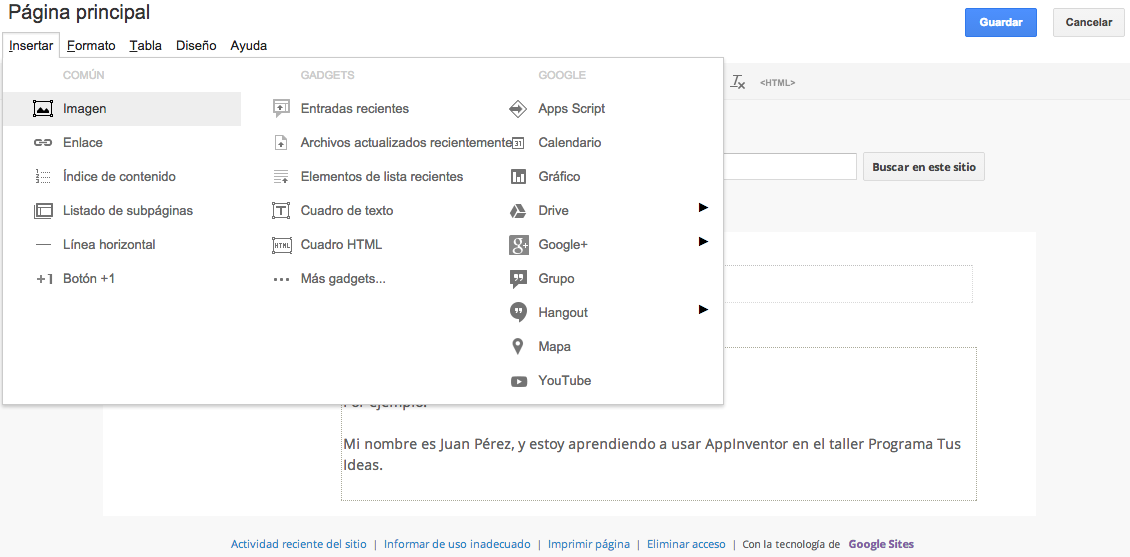
\includegraphics[scale=0.25]{SiteAddImage1}
\caption{Insertar imagen en tu sitio}
\label{fig:SiteAddImage1}
\end{figure}

\item Luego aparecerá una ventana como se muestra en
  la~\Cref{fig:SiteAddImage3}. Selecciona la opción ``Dirección web
  (URL)'', y pega desde el portapapeles la dirección que copiaste en
  el paso anterior.

\begin{figure}[H]
\centering
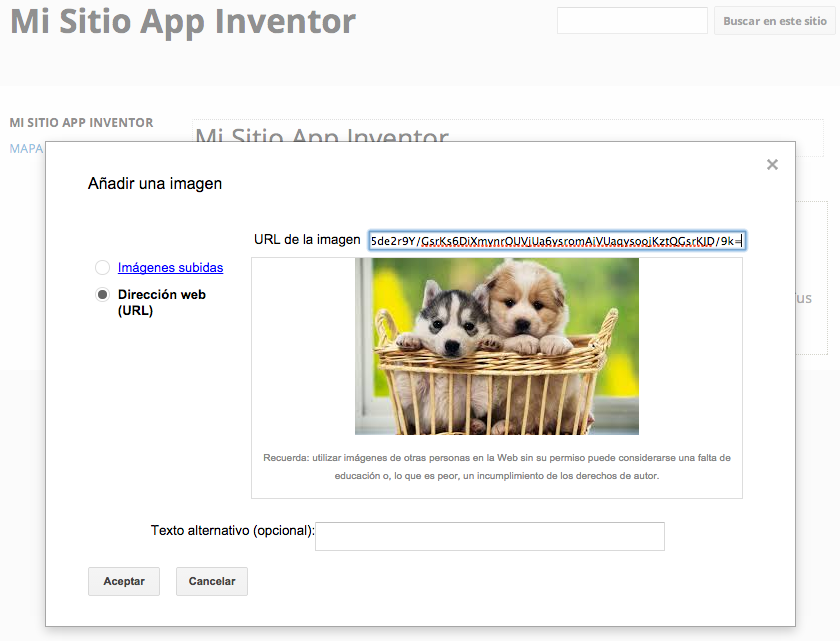
\includegraphics[scale=0.25]{SiteAddImage3}
\caption{Insertar imagen desde la Web, usando su URL}
\label{fig:SiteAddImage3}
\end{figure}

\item También puedes insertar una imagen que esté en tu
  computador. Para ello debes seleccionar la opción ``Imágenes
  subidas'' en la ventana del punto anterior, y subir la imagen que
  desees utilizar.

\item Personaliza el Sidebar (barra lateral) de tu sitio. El sidebar
  aparece en todos las páginas de tu sitio, y puedes personalizarlo
  para incluir diferentes elementos y enlaces. Sal del modo de edición
  y selecciona el botón de opciones (el que tiene un engranaje). Ahí
  selecciona la opción ``Modificar el diseño del sitio'', tal como se
  muestra en la~\Cref{fig:SiteSidebar1}.

\begin{figure}[H]
\centering
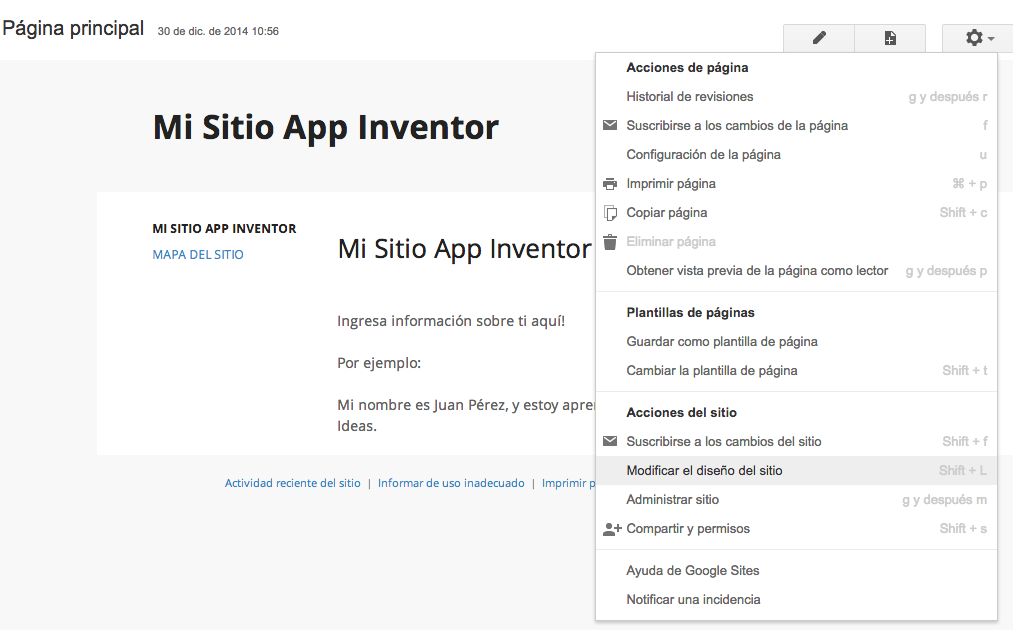
\includegraphics[scale=0.25]{SiteSidebar1}
\caption{Selecciona la opción para modificar el diseño del sitio}
\label{fig:SiteSidebar1}
\end{figure}

\item Ahora la barra lateral estará destacada, y tendrá dos botones:
  uno para edición (con un lápiz), y uno para agregar elementos (con
  un signo +). Al agregar un elemento al sidebar, aparecerá una nueva
  ventana como se muestra en la~\Cref{fig:SiteSidebar2}.

\begin{figure}[H]
\centering
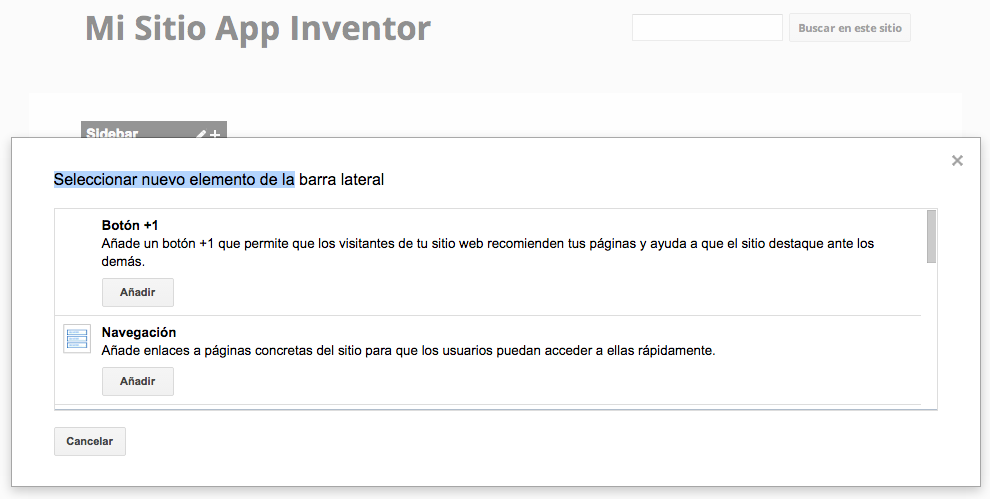
\includegraphics[scale=0.25]{SiteSidebar2}
\caption{Agregando un nuevo elemento al sidebar}
\label{fig:SiteSidebar2}
\end{figure}

\item Para subir archivos a tu sitio, selecciona nuevamente el menú
  del sitio (como lo hiciste para modificar el diseño del sitio) y
  escoge la opción ``Administrar sitio''. Entre las opciones que
  aparecerán escoge ``Archivos adjuntos''. Ahí podras subir, mover y
  eliminar los archivos que puedes poner a disposición de los
  visitantes a tu sitio, tal como se muestra en
  la~\Cref{fig:SiteFiles}.

\begin{figure}[H]
\centering
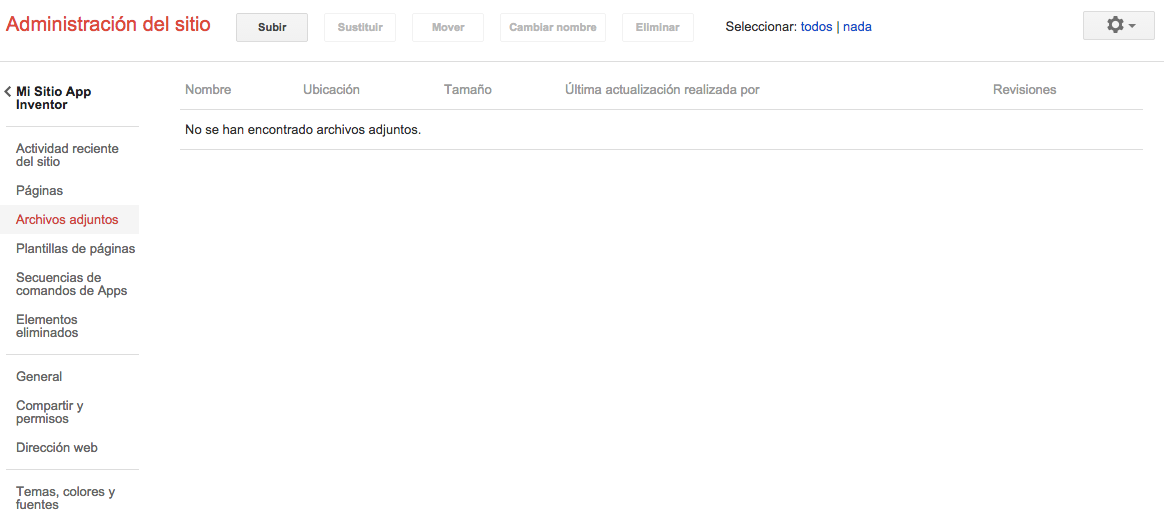
\includegraphics[scale=0.25]{SiteFiles}
\caption{Administrando los archivos adjuntos de tu sitio}
\label{fig:SiteFiles}
\end{figure}



\item Te invitamos a que descubras el potencial de Google Sites para
  diseñar tu portafolio. Recuerda que cualquier duda o problema lo
  puedes resolver con tu tutor!

\end{enumerate}

\section{Proyecto: Botonera de Sonidos}
\label{sec:proy-boton-de}

La actividad final del primer día de este taller consiste en que
realices tu propio proyecto, con un poquito de ayuda inicial. La meta
es que desarrolles una aplicación estilo ``botonera de sonidos'', que
consiste en múltiples botones que al ser presionados emiten distintos
sonidos. Para ayudarte un poco, hemos desarrollado una versión
preliminar de la aplicación que puedes descargar desde
\resources{ProgramaTusIdeas/Dia1/BotoneraSonidos/BotoneraSonidos.aia}. Luego
debes importar este proyecto en \AppInventor.

\paragraph{Interfaz de Usuario}

La~\Cref{fig:botoneraUI} muestra la interfaz de usuario de la
aplicación, que consiste en dos botones. A diferencia de \appName{Hola
  Gatito}, estamos usando un componente de \component{Disposición}
para ordenar los botones en la pantalla. Específicamente usamos una
\component{DisposiciónTabular} que crea una rejilla donde pueden
ponerse otros componentes.

\begin{figure}[H]
\centering
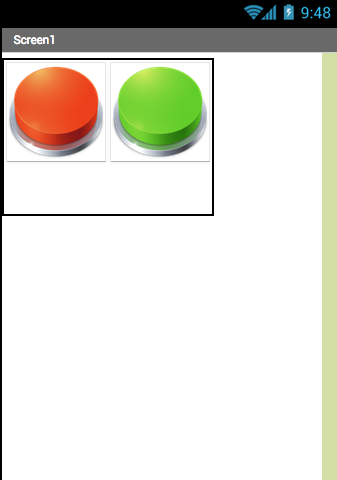
\includegraphics[scale=0.25]{BotoneraUI}
\caption{Interfaz de usuario de la plantilla para la botonera de sonidos}
\label{fig:botoneraUI}
\end{figure}

\paragraph{Comportamiento}

El código de la aplicación se muestra en
la~\Cref{fig:botoneraCode}. El código es muy similar al de
\appName{Hola Gatito}, pero tiene una diferencia fundamental. La
aplicación tiene sólo 1 componente \component{Sonido}, que se usa para
reproducir los sonidos de cada botón. Esto se logra cambiando la
propiedad \property{Origen} de forma \emph{dinámica}, dependiendo del
botón que es presionado. Para cambiar el origen del sonido, se
especifica el nombre del archivo a utilizar (que debe estar subido con
anterioridad).

\begin{figure}[H]
\centering
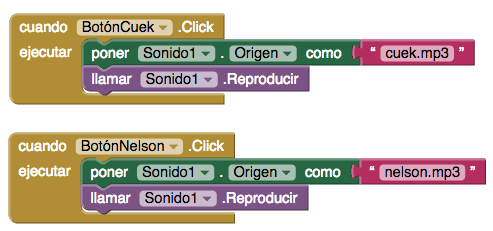
\includegraphics[scale=0.25]{BotoneraCode}
\caption{Código de la plantilla para la botonera de sonidos}
\label{fig:botoneraCode}
\end{figure}

\paragraph{Requerimientos del Proyecto}

Puedes crear la aplicación que quieras basándote en la idea y
plantilla originales. Sin embargo tu aplicación debiera cumplir al
menos los siguientes requerimientos:

\begin{itemize}

\item Debe tener una interfaz de usuario compleja, usando los
  componentes de \component{Disposición}.

\item Debe tener al menos cuatro sonidos que se reproduzcan en
  respuesta a distintos eventos (por ejemplo, presionar botones,
  agitar dispositivo, recibir mensajes de texto, etc.)

\item Debe tener algun comportamiento condicional, usando bloques
  \block{si, sino}.

\end{itemize}

\paragraph{Ideas} Algunas ideas para ayudarte con tu proyecto:

\begin{itemize}

\item Puedes encontrar y descargar sonidos desde internet, por ejemplo
  en \url{http://www.myinstants.com/}.

\item Reproducir notas de tus canciones favoritas, discursos, o charlas.

\item Software educacional para niños, por ejemplo una aplicación con
  los sonidos de una granja.

\item Un juego donde hay que descubrir el nombre de la canción. Al
  presionar el botón se escucha una parte de la canción, y al
  presionar otro botón se muestra el nombre de la canción.

\item Una aplicación que hace cosas diferentes cuando recibe mensajes
  de texto desde otro teléfono.

\item Una aplicación que te permite presionar las fotos de tus
  compañeros para ver sus nombres y escuchar sus voces.

\end{itemize}

\section{Material de Apoyo}
\label{sec:material-de-apoyo}

\subsection*{Entendiendo la Arquitectura de una Aplicación}

Muchas personas pueden decir qué es lo que es una aplicación, desde la
perspectiva del usuario, pero entender qué es una aplicación desde la
perspectiva de un \textit{\textbf{programador}} es más complicado. Las
aplicaciones tienen una estructura interna, lo que se conoce como la
\emph{arquitectura de la aplicación}, que se debe entender para poder
crear aplicaciones de manera efectiva.

Una manera de describir el interior de una aplicación es separarla en
dos partes: sus \emph{componentes}, y sus \emph{comportamientos}. En
general, estos conceptos corresponden a las dos ventanas principales
de \AppInventor. Por un lado, se usa el \componentDesigner para
especificar los componentes (u objetos) de la aplicación, y por otro
lado se usa el \blockEditor para programar cómo la aplicación responde
al usuario y a otros eventos externos. O sea, el \blockEditor se usa
para programar el comportamiento de la aplicación. La~\Cref{fig:appArchitecture}
muestra una vista general de la arquitectura de una aplicación.

\begin{figure}[H]
\centering
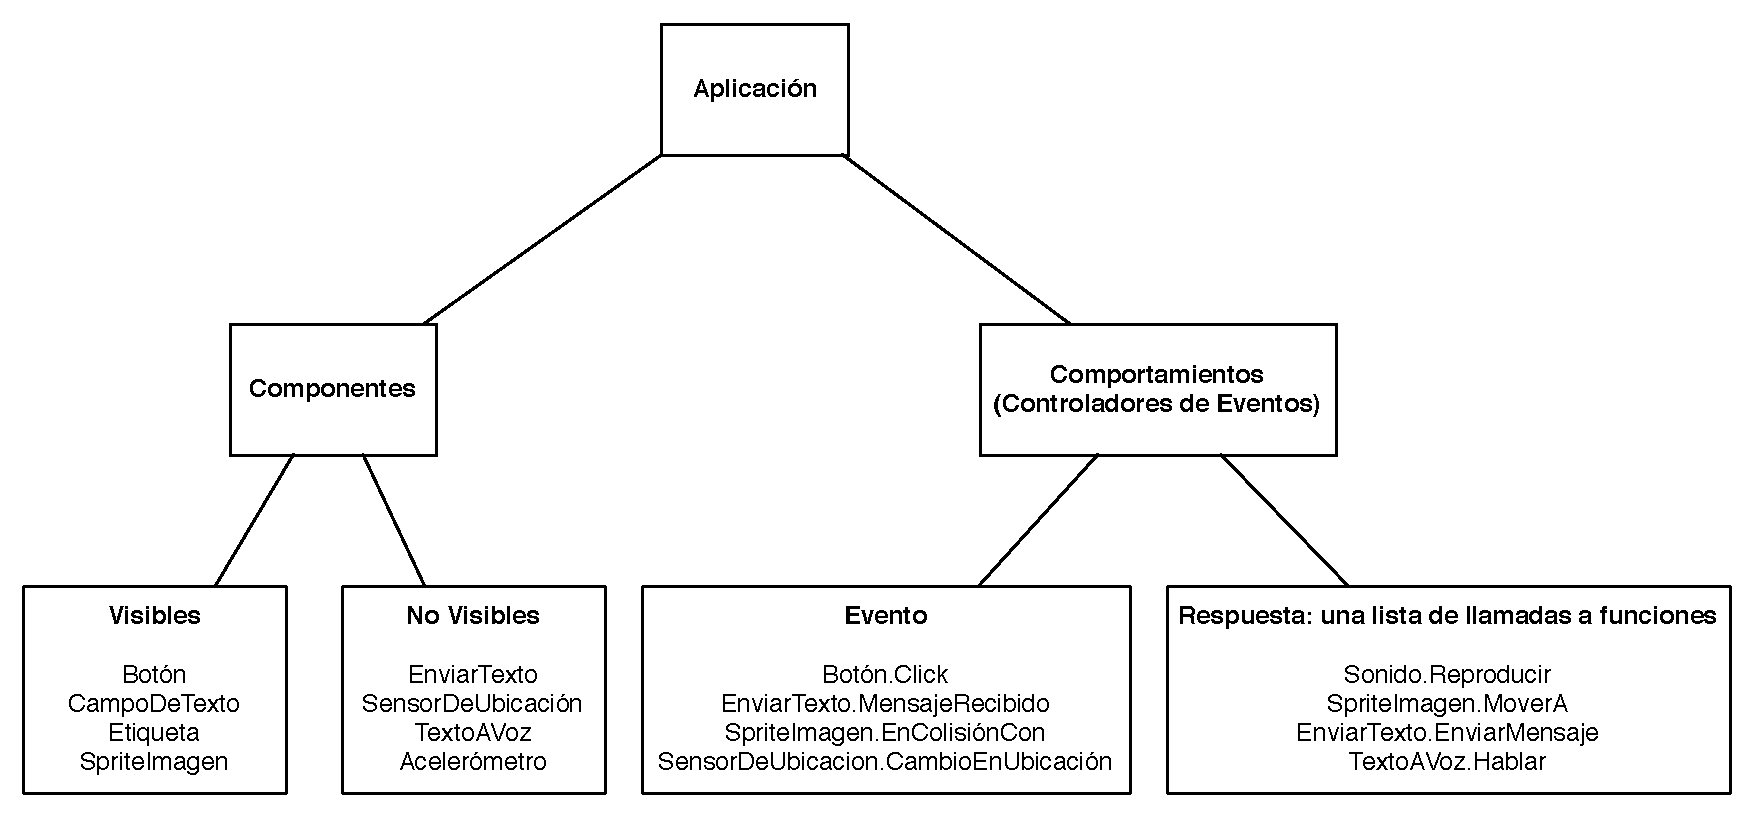
\includegraphics[scale=0.5]{AppArchitecture}
\caption{Arquitectura de una Aplicación: Componentes y Comportamiento}
\label{fig:appArchitecture}
\end{figure}

\subsubsection*{Componentes}

Existen dos tipos principales de componentes en una aplicación:
\emph{visibles} y \emph{no-visibles}. Los componentes visibles de una
aplicación son aquellos que se pueden ver cuando la aplicación se
ejecuta, por ejemplo los botones, cajas de texto y etiquetas. Al
conjunto de componentes visibles de una aplicación también se le
conoce como la \emph{interfaz de usuario}.

Los componentes no-visibles son aquellos que no se pueden ver, y que
por lo tanto no son parte de la interfaz de usuario. Su propósito es
proveer acceso a las funcionalidad preexistentes de un
dispositivo. Por ejemplo, el componente \component{EnviarTexto} envía
y procesa los mensajes de texto (SMS), el componente
\component{SensorDeUbicación} determina la ubicación del dispositivo,
y el componente \component{TextoAVoz} habla un mensaje escrito como
texto. Los componentes no-visibles representan la tecnología del
dispositivo que está a disposición del programador.

Tanto los componentes visibles como no-visibles se definen por un
conjunto de \emph{propiedades}. Las propiedades son espacios de
memoria para almacenar información sobre el componente. Los
componentes visibles, tales como botones o etiquetas, tienen
propiedades como su anchura, altura y alineamiento, los que en
conjunto definen cómo luce el componente.
%
Las propiedades de un componente son como celdas de una hoja de
cálculo. El programador las modifica en el \componentDesigner para
definir la apariencia \emph{inicial} del componente. También es
posible utilizar bloques para cambiar estos valores durante la
ejecución de la aplicación.

\subsubsection*{Comportamiento}

Los componentes de una aplicación son generalmente sencillos de
comprender, por ejemplo un campo de texto se usa para ingresar
información o un botón se usa para ser presionado. En cambio, el
comportamiento de una aplicación es conceptualmente difícil y a menudo
complejo. El comportamiento define cómo la aplicación debiera
responder a eventos, tanto eventos iniciados por el usuario (por
ejemplo, se presiona un botón) como eventos externos (por ejemplo, se
recibió un mensaje de texto). La dificultad de especificar ese
comportamiento interactivo es el por qué la programación es un
desafío.

Afortunadamente, \AppInventor provee un lenguaje de \emph{bloques}
para especificar estos comportamientos. Los bloques hacen que
programar el comportamiento sea similar a juntar las piezas de un
puzzle, en contraste a recordar y escribir código como en lenguajes de
programación tradicionales. Además, \AppInventor está diseñado para
especificar comportamientos en respuesta a eventos de una manera
sencilla y directa.

\subsubsection*{Una Aplicación es Como una Receta de Cocina}

Tradicionalmente se ha comparado al software (programas, aplicaciones)
con una receta de cocina. Como en una receta, una aplicación
tradicional sigue una secuencia lineal de instrucciones, como las de
la~\Cref{fig:lineal}, que el computador debiera ejecutar.

\begin{figure}[H]
\centering
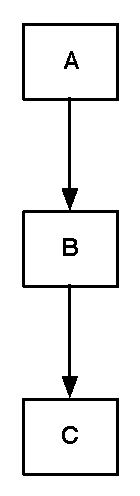
\includegraphics[scale=0.5]{Lineal}
\caption{Una aplicación tradicional sigue una serie de pasos
  secuenciales, como una receta de cocina.}
\label{fig:lineal}
\end{figure}

Si consideramos como ejemplo una aplicación de un cajero automático,
una primera operación (A) sería iniciar una transacción bancaria,
luego (B) especificar el monto que se desea retirar, y finalmente (C)
modificar la cuenta del cliente, entregar el dinero y luego imprimir
el saldo por pantalla.

\subsubsection*{Una Aplicación Como un Conjunto de Controladores de
  Eventos}

La visión de una aplicación como una receta de cocina calza bien con
las aplicaciones o programas que se hacían en los inicios de la
computación, pero no es una gran idea para la programación de
dispositivos móviles, ni en la Web, ni en la mayoría de las
aplicaciones y plataformas actuales en computación. La mayor parte del
software moderno no realiza un puñado de instrucciones en un orden
predeterminado. Lo que se hace es que el software \emph{reaccione}
ante distintos \emph{eventos}---la mayoría iniciados por la
interacción entre el usuario y la aplicación (por ejemplo, abrir un
video en Youtube).

En el caso de las aplicaciones móviles tenemos diversos eventos
gatillados por el usuario. Por ejemplo, al presionar el botón
``Enviar'', la aplicación responde enviando un mensaje de texto. El
deslizar el dedo por la pantalla táctil también es otro evento. La
aplicación podría responder dibujando una línea entre el punto donde
se comenzó a deslizar el dedo y el punto donde se levantó.

Considerando lo anterior, las aplicaciones modernas se pueden entender
mejor como máquinas de eventos-respuestas. Ocurre que las aplicaciones
igual incluyen “recetas”—secuencias de instrucciones—pero la
diferencia es que cada receta es realizada sólo en respuesta a algún
evento en particular. La~\Cref{fig:eventHandlers} ilustra esta idea.

\begin{figure}[H]
\centering
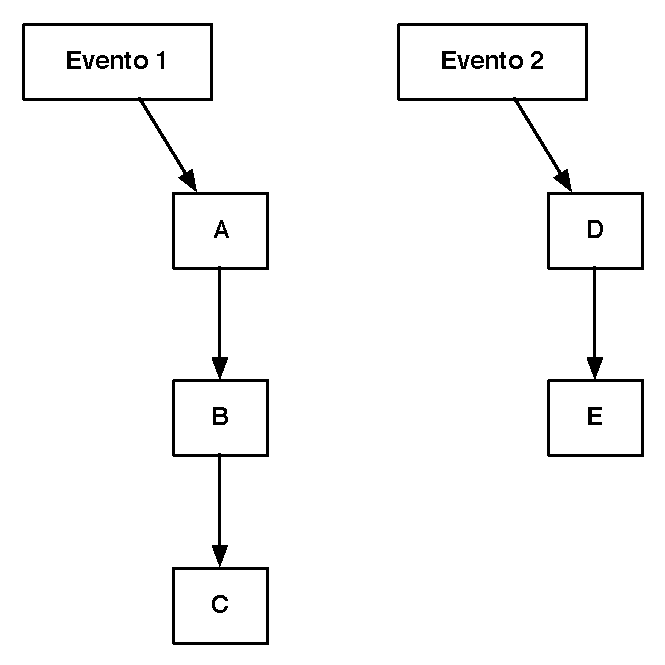
\includegraphics[scale=0.5]{EventHandlers}
\caption{Una aplicación consiste en un conjunto de controladores de eventos.}
\label{fig:eventHandlers}
\end{figure}

A medida que los eventos ocurren, la aplicación reacciona ejecutando
una secuencia de funciones. Las funciones son cosas que se pueden
hacer con un componente (o hacia un componente), como mandar un
mensaje de texto o cambiar la propiedad de algún componente (por
ejemplo, cambiar el texto de un botón en la interfaz de
usuario). \emph{Llamar} a una función significa invocar a esa función,
o sea hacer que ocurra lo que esa función hace. Usaremos el término
\emph{controlador de eventos} para referirnos tanto a un evento como
al conjunto de funciones que se ejecutan como respuesta.

Muchos eventos son iniciados por el usuario, pero algunos no lo
son. Una aplicación puede reaccionar a eventos que ocurren al
\emph{interior del teléfono}, tales como cambios en su sensor de
orientación o su reloj (o sea, respecto al paso del tiempo), y también
a eventos creados por cosas \emph{externas al teléfono}, tales como la
recepción de un mensaje de texto o una llamada telefónica, o la
llegada de datos desde la Web. Esto se muestra en
la~\Cref{fig:events}.

\begin{figure}[H]
\centering
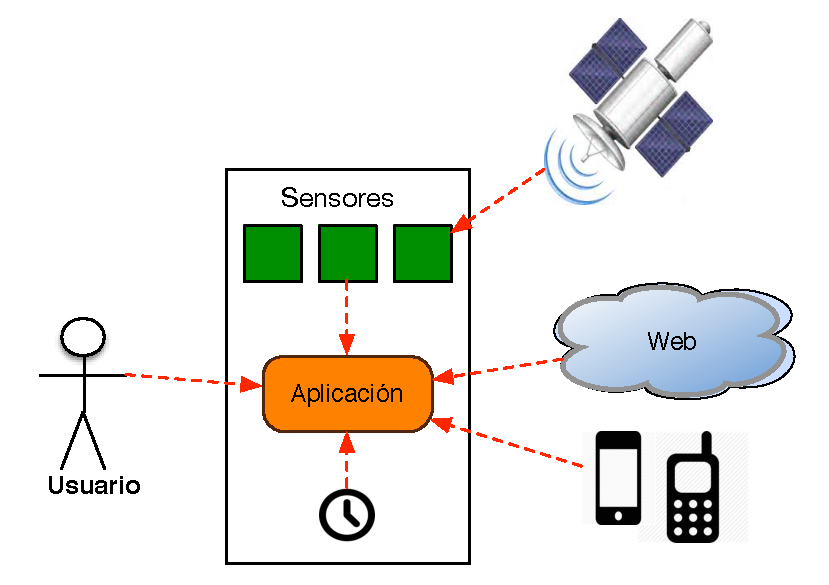
\includegraphics[scale=0.5]{Events}
\caption{Eventos internos y externos al teléfono.}
\label{fig:events}
\end{figure}

Una razón por la cual la programación en \AppInventor es intuitiva es
porque se basa directamente en este modelo evento-respuesta. Una
aplicación se comienza a programar arrastrando un bloque de evento, el
cual tiene la forma ``\emph{Cuando} ... \emph{ejecutar} ...''. Por ejemplo,
consideremos una aplicación que responde al evento de presionar un
botón leyendo el texto que el usuario a ingresado en una caja de
texto, se programa con un único controlador de eventos, como se
muestra en la~\Cref{fig:speakit1}.

\begin{figure}[H]
\centering
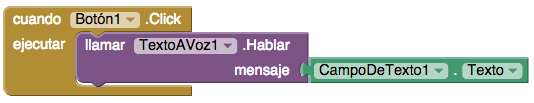
\includegraphics[scale=0.5]{SpeakIt1}
\caption{Código para hablar texto ingresado por el usuario.}
\label{fig:speakit1}
\end{figure}

Estos bloques especifican que cuando el usuario presiona el
\component{Botón1}, el componente \component{TextoAVoz} debiera hablar
las palabras que el usuario ha ingresado en el
\component{CampoDeTexto1}. La respuesta al evento
\component{Botón1.Click} es la llamada a la función
\component{TextoAVoz.Hablar}. El controlador del evento son todos los
bloques de la figura.

En \AppInventor, todas las actividades ocurren en respuesta a algún
evento. Por lo tanto una aplicación no debiera contener bloques que
estén afuera de un bloque “Cuando-ejecutar”. Por ejemplo, no tiene
sentido que los bloques de la~\Cref{fig:speakit2} estén flotando solos
en el editor de bloques.

\begin{figure}[H]
\centering
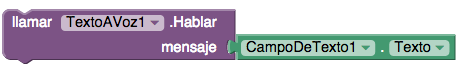
\includegraphics[scale=0.5]{SpeakIt2}
\caption{Las respuestas deben ir asociadas a un controlador de eventos.}
\label{fig:speakit2}
\end{figure}

\subsubsection*{Tipos de Eventos}

La~\Cref{tab:eventTypes} resume los tipos de eventos existentes en las
aplicaciones \AppInventor. A continuación describiremos cada uno de
ellos.

\begin{table}[H]
\begin{small}
\begin{tabular}{|l|l|}
  \hline
  \textbf{Tipo de Evento} & \textbf{Ejemplo}\\
  \hline
  Evento iniciado por el usuario & \emph{Cuando} el usuario presiona
  Botón1, \emph{realizar} ...\\
  \hline
  Evento de inicialización & \emph{Cuando} la aplicación se empieza a
  ejecutar, \emph{realizar} ...\\
  \hline
  Evento de temporizador & \emph{Cuando} pasen 20 milisegundos,
  \emph{realizar} ...\\
\hline
Evento de animación & \emph{Cuando} dos objetos colisionen,
\emph{realizar} ...\\
\hline
Evento externo & \emph{Cuando} el teléfono recibe un mensaje de texto,
\emph{realizar} ...\\
\hline
\end{tabular}
\end{small}
\caption{Tipos de Eventos}
\label{fig:eventTypes}
\end{table}

\paragraph{Eventos iniciados por el usuario}
Los eventos iniciados por el usuario son el tipo de evento más
común. Con aplicaciones tipo ``trivia'', el presionar botones es la
manera usual de gatillar respuestas de la aplicación. Otras
aplicaciones más gráficas responden a toques en la pantalla y a
arrastrar elementos por la misma.

\paragraph{Eventos de inicialización}
Algunas veces una aplicación necesita realizar ciertas funciones justo
cuando la aplicación comienza, y no en respuesta a alguna actividad
del usuario final. Para este propósito, \AppInventor considera el
“lanzar” la aplicación como un evento. Por lo tanto, si el programador
lo requiere, se pueden especificar funciones para ser ejecutadas
inmediatamente una vez que la aplicación se abre. Para ello se utiliza
el bloque \component{Screen1.Inicializar}. En el juego \emph{Atrapa el
  Topo}, que se realizará el segundo día se utilizará este evento para
asignar una posición inicial al azar a un elemento del juego, de forma
similar al código de la~\Cref{fig:initialize}.

\begin{figure}[H]
\centering
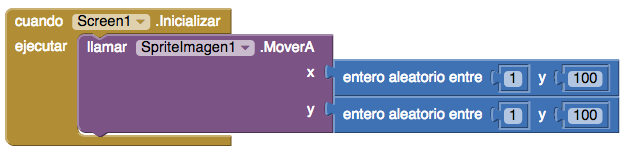
\includegraphics[scale=0.5]{Initialize}
\caption{Asignando una posición al azar al inicio de la aplicación.}
\label{fig:initialize}
\end{figure}

\paragraph{Eventos de temporizador}
Algunas actividades de una aplicación son gatilladas por el paso del
tiempo. Por ejemplo, uno puede considerar que una animación es un
objeto que se mueve gatillado por un evento de
temporizador. \AppInventor tiene un componente \component{Reloj} que
se usa para gatillar eventos de temporizador. Por ejemplo, el código
para mover una pelota por la pantalla 10 pixeles horizontalmente cada
cierto intervalo de tiempo es similar al de la~\Cref{fig:clockEvent}.

\begin{figure}[H]
\centering
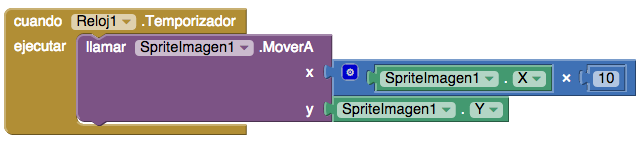
\includegraphics[scale=0.5]{ClockEvent}
\caption{Animación gatillada por el reloj.}
\label{fig:clockEvent}
\end{figure}

\paragraph{Eventos de animación}
Las actividades que involucran objetos gráficos (sprites) dentro de
lienzos gatillarán eventos. Por lo tanto es posible programar juegos y
otras aplicaciones interactivas especificando qué debiera ocurrir en
eventos tales como un objeto alcanzando el borde del lienzo, o la
colisión de dos objetos. Un código de ejemplo de colisión se muestra
en la~\Cref{fig:colision}.

\begin{figure}[H]
\centering
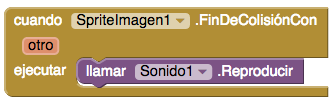
\includegraphics[scale=0.5]{Colision}
\caption{Controlador de eventos para la colisión entre dos objetos de
  un juego.}
\label{fig:colision}
\end{figure}

\paragraph{Eventos externos}

Cuando el teléfono recibe información GPS sobre su ubicación también
se gatilla un evento. Lo mismo pasa cuando el teléfono recibe un
mensaje de texto, por ejemplo, el código para una respuesta automática
a un mensaje de texto recibido se muestra en la~\Cref{fig:autoreply}.

\begin{figure}[H]
\centering
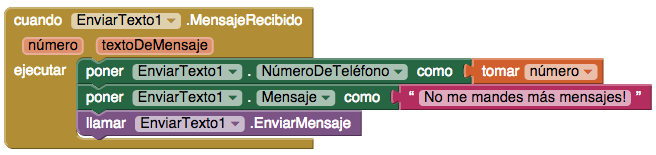
\includegraphics[scale=0.5]{AutoReply}
\caption{Respuesta automática a un mensaje de texto.}
\label{fig:colision}
\end{figure}

Todos los tipos de eventos se consideran de la misma forma que
cualquier otro. En conclusión, cada aplicación creada usando
\AppInventor consiste en un conjunto de controladores de eventos:
algunos para inicializar cosas, otros para responder al usuario, otros
gatillados por el tiempo, y otros gatillados por eventos externos. Tu
trabajo como programador es conceptualizar tu aplicación de esta
manera, y diseñar la respuesta de cada controlador de eventos
relevante para tu aplicación.

\subsubsection*{Los Controladores de Eventos pueden Hacer Preguntas}
Las respuestas a los eventos no siempre siguen recetas de cocina
secuenciales, sino que es posible hacer preguntas y repetir
operaciones. ``Hacer preguntas'' significa consultar los datos
almacenados en la aplicación y determinar el curso de acción (o
\emph{rama} de acción) dependiendo de las respuestas a estas
consultas. En estos casos decimos que la aplicación tiene \emph{ramas
  condicionales}, como se ilustra en la~\Cref{fig:conditionals}.

\begin{figure}[H]
\centering
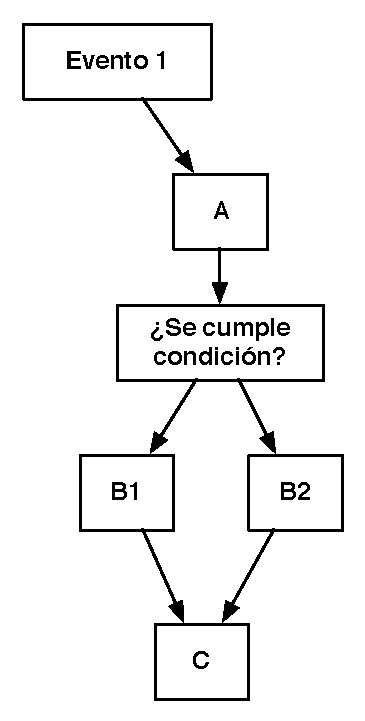
\includegraphics[scale=0.5]{Conditionals}
\caption{Aplicación con ramas condicionales de ejecución.}
\label{fig:conditionals}
\end{figure}

Las pruebas condicionales son preguntase tales como ``¿Llegó el
puntaje a 100?'', o ``¿El mensaje de texto recién recibido fue enviado
por Juan?''.  Las preguntas pueden incluir fórmulas complejas que
incluyen comparadores algebraicos (menor que, mayor que, igual a) y
lógicos (“y”, “o”, “no”). Los comportamientos condicionales en
\AppInventor se especifican usando bloques \block{si, sino}. Por
ejemplo, los bloques de la~\Cref{fig:score} reportarán el mensaje
``Ganaste!'' si el jugador tiene más de 100 puntos.

\begin{figure}[H]
\centering
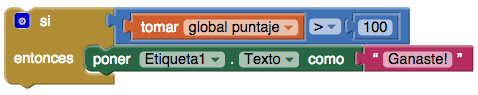
\includegraphics[scale=0.5]{Score}
\caption{Preguntar si el puntaje es superior a 100.}
\label{fig:score}
\end{figure}

\subsubsection*{Los Controladores de Eventos pueden Repetir Operaciones}
Además de hacer preguntas y ejecutar distintas recetas según cada
caso, una respuesta a un evento puede también incluir repeticiones de
operaciones múltiples veces. \AppInventor provee diversos bloques para
especificar tales operaciones, tales como \block{por cada} y
\block{mientras-comprobar-ejecutar}, los cuales encierran una
secuencia de bloques cuya ejecución se repetirá. Todos los bloques
dentro de un \block{por cada} se ejecutan una vez para cada elemento
en una \emph{lista}. Por ejemplo, el código enviar un mensaje de texto a
una lista de números de teléfono es similar al de
la~\Cref{fig:foreach}.

\begin{figure}[H]
\centering
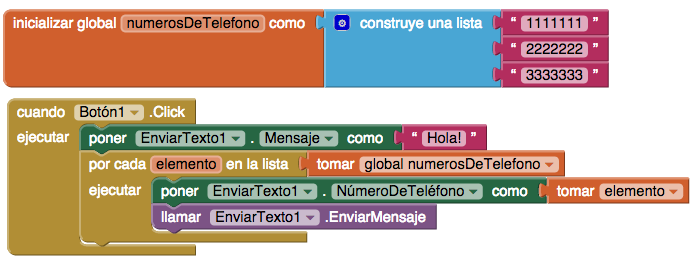
\includegraphics[scale=0.5]{Foreach}
\caption{Usar repetición para enviar un mensaje de texto a cada
  teléfono en una lista.}
\label{fig:foreach}
\end{figure}

\subsubsection*{Los Controladores de Eventos pueden Recordar Cosas}

A menudo un controlador de eventos necesita hacer un seguimiento de la
información a medida que ejecuta sus bloques. Esta información puede
almacenarse en ubicaciones de memoria conocidas como \emph{variables}, las
cuales se definen en el \blockEditor. De hecho, en las secciones
anteriores ya hemos visto el uso de variables para almacenar el
puntaje de un juego y para definir una lista de números de teléfono.

Las variables son como las propiedades, pero no están asociadas a
ningún componente en particular. En un juego, por ejemplo, se puede
definir una variable puntaje la cual será modificada por los
controladores de eventos según la lógica propia de cada juego. Las
variables almacenan los datos de manera temporal, mientras la
aplicación se está ejecutando; pero cuando se cierra la aplicación los
datos dejan de estar disponibles.

A veces una aplicación necesita recordar cosas no sólo mientras se
ejecuta, sino incluso cuando es cerrada y vuelta a abrir. Por ejemplo
para mantener un historial de los mayores puntajes, es necesario
almacenar esta información a largo plazo, de manera que esté
disponible la próxima vez que alguien juegue a este juego. Los datos
que se mantienen incluso después de que una aplicación se cierra se
llaman \emph{datos persistentes}, y se almacenan en algún tipo de base
de datos. En los siguientes días del taller profundizaremos más sobre
el uso de variables y de datos persistentes.

\end{document}
